% !TeX program = xelatex
% Author: Mark H. Olson
% Website: https://mholson.com
% Github: https://github.com/mholson

%=+=+=+=+=+=+=+=+=+=+=+=+=+=+=+=+=+=+=+=+=+=+=+=+=+=+=+=+=+=+=+=+=+=+=+=+=+=+=+=

%=-=-=-=-=-=-=-=-=-=-=-=-=-=-=-=-=-=-=-=-=-=-=-=-=-=-=-=-=-=-=-=-=-=-=-=-=-=-=-=
% PREAMBLE :: sthlmNordLightDemo.tex 
%=-=-=-=-=-=-=-=-=-=-=-=-=-=-=-=-=-=-=-=-=-=-=-=-=-=-=-=-=-=-=-=-=-=-=-=-=-=-=-=
%
% > > >	The following beamer class options are available
%		aspectratio=169		Change aspect ratio to 16:9	
%		bibref				Include bibliography
%		sectionpages		Show section pages
%		codeminted			use minted pkg for code printing instead of listings
%							(requires additional setup & Python installed)
% 		font sizes 			{8, 9, 10, 11, 12, 14, 17, 20} 11 Default
%
% > > > The following sthlmnord package options are available
%		mode				= dark (default)
%							= light
%=-=-=-=-=-=-=-=-=-=-=-=-=-=-=-=-=-=-=-=-=-=-=-=-=-=-=-=-=-=-=-=-=-=-=-=-=-=-=-=

\documentclass[usenames,11,dvipsnames,svgnames,x11names,aspectratio=1610,bibref]{beamer}
% > > > Bibliography File 
\newcommand{\bibfilename}{mhoreferences.bib}
% > > > Choose Theme
\usetheme[mode=light]{sthlmnord}
%\usetheme{sthlmnord}

\usepackage[normalem]{ulem}                 % \uline
\usepackage{multicol}
\usepackage{tikz}
% \usepackage[]{roboto-mono}
% \usepackage{enumitem}
\usepackage{xspace}
\usepackage{awesomebox}
% \usepackage[font=scriptsize,labelfont=bf]{caption}
\usepackage{subcaption} % for captionof
% \usepackage{cleveref}

% \usepackage{titlesec} % paragraph symbol \S
\usepackage{underscore}                     % to write underscores without escaping them
\usepackage[minted,listings]{tcolorbox}     % listing
\usepackage{minted}

\usemintedstyle{tango}
\usepackage{xparse}

\usepackage{paralist}                       % compactitem, compactenum


\usepackage{fontawesome5}

\newcommand{\cmark}{\ding{51}}%
\newcommand{\xmark}{\ding{55}}%


\newcommand{\myimportantbox}[1]{%
  \awesomebox[nordEleven]{2pt}{\faFire}{nordEleven}{#1}}
  
\newcommand{\mytipbox}[1]{%
  \awesomebox[nordEleven!50]{2pt}{\faLightbulb[regular]}{Tomato}{#1}}

%%%%%%%%%%%%%%%%%%%%%%%%%%%%%%%%%%%
% FONTS
%%%%%%%%%%%%%%%%%%%%%%%%%%%%%%%%%%%
\newfontfamily{\orbitron}{orbitron}[
    Path=./fonts/orbitron/,
    Extension = .otf,
    UprightFont = *-light,
    BoldFont = *-medium
    ]
    
\newfontfamily{\robotomono}{robotomono}[
    Path=./fonts/robotomono/,
    Extension = .ttf,
    UprightFont = *-Regular,
    BoldFont = *-Bold,
    BoldItalicFont = *-BoldItalic,
    ItalicFont = *-Italic,
    NFSSFamily=RobotoMonoFamily
    ]

% \newfontfamily\monaco{Arial}[NFSSFamily=ArialFamily]
% \setminted[matlab]{fontfamily=ArialFamily}

% \newfontfamily{\raleway}{Raleway}[
%     Path=./fonts/raleway/,
%     Extension = .ttf,
%     UprightFont = *-Medium,
%     BoldFont = *-Bold,
%     BoldItalicFont = *-BoldItalic,
%     ItalicFont = *-Italic
%     ]


    
    
    
% \newfontfamily{\ralewayII}{Raleway}[
%     Path=./fonts/raleway/,
%     Extension = .ttf,
%     UprightFont = *-Light,
%     BoldFont = *-SemiBold,
%     BoldItalicFont = *-SemiBoldItalic,
%     ItalicFont = *-LightItalic
%     ]

% \newfontfamily{\ralewayIII}{Raleway}[
%     Path=./fonts/raleway/,
%     Extension = .ttf,
%     UprightFont = *-Thin,
%     BoldFont = *-Bold,
%     BoldItalicFont = *-BoldItalic,
%     ItalicFont = *-Italic
%     ]
    


%%%%%%%%%%%%%%%%%%%%%%%%%%%%%%%%%%%
% code error
%%%%%%%%%%%%%%%%%%%%%%%%%%%%%%%%%%%
\definecolor{coderror}{HTML}{f06b6b}
\newcommand{\codeerror}{\textcolor{coderror}{\bf error}}
\newcommand{\codeerrorII}[1]{\textcolor{coderror}{\bf #1}}
%%%%%%%%%%%%%%%%%%%%%%%%%%%%%%%%%%%
% VINIK24 colors
%%%%%%%%%%%%%%%%%%%%%%%%%%%%%%%%%%%


% 000000
% 6f6776
% 9a9a97
% c5ccb8
% 8b5580
% c38890
% a593a5
% 666092
% 9a4f50
% c28d75
% 7ca1c0
% 416aa3
% 8d6268
% be955c
% 68aca9
% 387080
% 6e6962
% 93a167
% 6eaa78
% 557064
% 9d9f7f
% 7e9e99
% 5d6872
% 433455

\definecolor{vinik1}{HTML}{000000}
\newcommand{\vinikI}[1]{\textcolor{vinik1}{#1}}
\definecolor{vinik2}{HTML}{6f6776}
\newcommand{\vinikII}[1]{\textcolor{vinik2}{#1}}
\definecolor{vinik3}{HTML}{9a9a97}
\newcommand{\vinikIII}[1]{\textcolor{vinik3}{#1}}
\definecolor{vinik4}{HTML}{c5ccb8}
\newcommand{\vinikIV}[1]{\textcolor{vinik4}{#1}}
\definecolor{vinik5}{HTML}{8b5580}
\newcommand{\vinikV}[1]{\textcolor{vinik5}{#1}}
\definecolor{vinik6}{HTML}{c38890}
\newcommand{\vinikVI}[1]{\textcolor{vinik6}{#1}}
\definecolor{vinik7}{HTML}{a593a5}
\newcommand{\vinikVII}[1]{\textcolor{vinik7}{#1}}
\definecolor{vinik8}{HTML}{666092}
\newcommand{\vinikVIII}[1]{\textcolor{vinik8}{#1}}
\definecolor{vinik9}{HTML}{9a4f50}
\newcommand{\vinikIX}[1]{\textcolor{vinik9}{#1}}
\definecolor{vinik10}{HTML}{c28d75}
\newcommand{\vinikX}[1]{\textcolor{vinik10}{#1}}
\definecolor{vinik11}{HTML}{7ca1c0}
\newcommand{\vinikXI}[1]{\textcolor{vinik11}{#1}}
\definecolor{vinik12}{HTML}{416aa3}
\newcommand{\vinikXII}[1]{\textcolor{vinik12}{#1}}
\definecolor{vinik13}{HTML}{8d6268}
\newcommand{\vinikXIII}[1]{\textcolor{vinik13}{#1}}
\definecolor{vinik14}{HTML}{be955c}
\newcommand{\vinikXIV}[1]{\textcolor{vinik14}{#1}}
\definecolor{vinik15}{HTML}{68aca9}
\newcommand{\vinikXV}[1]{\textcolor{vinik15}{#1}}
\definecolor{vinik16}{HTML}{387080}
\newcommand{\vinikXVI}[1]{\textcolor{vinik16}{#1}}
\definecolor{vinik17}{HTML}{6e6962}
\newcommand{\vinikXVII}[1]{\textcolor{vinik17}{#1}}
\definecolor{vinik18}{HTML}{93a167}
\newcommand{\vinikXVIII}[1]{\textcolor{vinik18}{#1}}
\definecolor{vinik19}{HTML}{6eaa78}
\newcommand{\vinikXIX}[1]{\textcolor{vinik19}{#1}}
\definecolor{vinik20}{HTML}{557064}
\newcommand{\vinikXX}[1]{\textcolor{vinik20}{#1}}
\definecolor{vinik21}{HTML}{9d9f7f}
\newcommand{\vinikXXI}[1]{\textcolor{vinik21}{#1}}
\definecolor{vinik22}{HTML}{7e9e99}
\newcommand{\vinikXXII}[1]{\textcolor{vinik22}{#1}}
\definecolor{vinik23}{HTML}{5d6872}
\newcommand{\vinikXXIII}[1]{\textcolor{vinik23}{#1}}
\definecolor{vinik24}{HTML}{433455}
\newcommand{\vinikXXIV}[1]{\textcolor{vinik24}{#1}}

\newcommand{\syntaxgray}[1]{\textcolor{vinik23}{#1}}


\definecolor{definitioncolor}{HTML}{3C415C}
\newcommand{\mydefinitioncolor}[1]{\textcolor{definitioncolor}{#1}}



\definecolor{sectionchevron}{HTML}{76BA99}
\newcommand{\sectionColor}[1]{\textcolor{sectionchevron}{#1}}

\definecolor{subsectionchevron}{HTML}{ADCF9F}
\newcommand{\subsectionColor}[1]{\textcolor{subsectionchevron}{#1}}

\definecolor{subsubsectionchevron}{HTML}{CED89E}
\newcommand{\subsubsectionColor}[1]{\textcolor{subsubsectionchevron}{#1}}

\definecolor{customcolor}{HTML}{A77979}
\definecolor{citationcolor}{HTML}{F67280}
\newcommand{\citationcolor}[1]{\textcolor{nordEleven}{#1}}




%%%%%%%%%%%%%%%%%%%%%%%%%%%%%%%%%%%
% CARNIVAL32 colors
%%%%%%%%%%%%%%%%%%%%%%%%%%%%%%%%%%%


% 000000
% 6f6776
% 9a9a97
% c5ccb8
% 8b5580
% c38890
% a593a5
% 666092
% 9a4f50
% c28d75
% 7ca1c0
% 416aa3
% 8d6268
% be955c
% 68aca9
% 387080
% 6e6962
% 93a167
% 6eaa78
% 557064
% 9d9f7f
% 7e9e99
% 5d6872
% 433455

\definecolor{carnival19}{HTML}{4d528a}
\newcommand{\carnivalXIX}[1]{\textcolor{carnival19}{#1}}
\newcommand{\monster}{\textbf{\textcolor{DodgerBlue1}{rpg::Monster}}}
\newcommand{\vampire}{\textbf{\textcolor{BurntOrange}{rpg::Vampire}}}
\newcommand{\werewolf}{\textbf{\textcolor{WildStrawberry}{rpg::Werewolf}}}


\definecolor{carnival20}{HTML}{556a97}
\newcommand{\carnivalXX}[1]{\textcolor{carnival20}{#1}}




\definecolor{carnival21}{HTML}{5c81a3}
\newcommand{\carnivalXXI}[1]{\textcolor{carnival21}{#1}}
\definecolor{carnival22}{HTML}{7dadc8}
\newcommand{\carnivalXXII}[1]{\textcolor{carnival22}{#1}}
\definecolor{carnival23}{HTML}{b0d6d9}
\newcommand{\carnivalXXIII}[1]{\textcolor{carnival23}{#1}}
\definecolor{carnival24}{HTML}{ece6df}
\newcommand{\carnivalXXIV}[1]{\textcolor{carnival24}{#1}}
\definecolor{carnival25}{HTML}{cfccca}
\newcommand{\carnivalXXV}[1]{\textcolor{carnival25}{#1}}




\definecolor{iconColor}{HTML}{383E56}
\definecolor{iconWarningColor}{HTML}{FA370E}
\definecolor{iconOkColor}{HTML}{00A8CC}
\definecolor{iconBestPracticeColor}{HTML}{00A8CC}
\newcommand{\iconColor}[1]{\textcolor{iconColor}{#1}}
\newcommand{\iconWarningColor}[1]{\textcolor{iconWarningColor}{#1}}
\newcommand{\iconBestPracticeColor}[1]{\textcolor{DodgerBlue}{#1}}

\newcommand{\iconOKColor}[1]{\textcolor{iconOkColor}{#1}}

\definecolor{codecolor1}{HTML}{004822}
\newcommand{\codecolorI}[1]{\textcolor{DeepPink1}{\bf #1}}
\definecolor{codecolor2}{HTML}{FD3135}
\newcommand{\codecolorII}[1]{\textcolor{DeepSkyBlue4}{\bf #1}}
\definecolor{codecolor3}{HTML}{0E6B8C}
\newcommand{\codecolorIII}[1]{\textcolor{IndianRed1}{\bf #1}}

%%%%%%%%%%%%%%%%%%%%%%%%%%%%%%%%%%%
% line number customized
\renewcommand{\theFancyVerbLine}{\textcolor{carnival19}{\sf\scriptsize\arabic{FancyVerbLine}}}
\newcommand{\myline}[1]{{\textcolor{carnival19}{#1}}}
%%%%%%%%%%%%%%%%%%%%%%%%%%%%%%%%%%%

%%%%%%%%%%%%%%%%%%%%%%%%%%%%%%%%%%%
% Directory tree
%%%%%%%%%%%%%%%%%%%%%%%%%%%%%%%%%%%
\usepackage[edges]{forest}

\newlength\Size
\setlength\Size{4pt}
\tikzset{%
  folder/.pic={%
  \node[inner sep=0pt] (folder) at (0.16,0)
    {\normalsize\textcolor{black}{\faFolderOpen}};
    % \filldraw [draw=folderborder, top color=folderbg!50, bottom color=folderbg] (-1.05*\Size,0.2\Size+5pt) rectangle ++(.75*\Size,-0.2\Size-5pt);
    % \filldraw [draw=folderborder, top color=folderbg!50, bottom color=folderbg] (-1.15*\Size,-\Size) rectangle (1.15*\Size,\Size);
  },
  file/.pic={%
  \node[inner sep=0pt] (file) at (0.13,0)
    {\normalsize\faFile*[regular]};
    % \filldraw [draw=folderborder, top color=folderbg!5, bottom color=folderbg!10] (-\Size,.4*\Size+5pt) coordinate (a) |- (\Size,-1.2*\Size) coordinate (b) -- ++(0,1.6*\Size) coordinate (c) -- ++(-5pt,5pt) coordinate (d) -- cycle (d) |- (c) ;
  },
}
\forestset{%
  declare autowrapped toks={pic me}{},
  declare boolean register={pic root},
  pic root=0,
  pic dir tree/.style={%
    for tree={%
      folder,
      font=\raleway,
      grow'=0,
      l=0,
    },
    before typesetting nodes={%
      for tree={%
        edge label+/.option={pic me},
        l=0,
      },
      if pic root={
        tikz+={
          \pic at ([xshift=\Size].west) {folder};
        },
        align={l}
      }{},
    },
  },
  pic me set/.code n args=2{%
    \forestset{%
      #1/.style={%
        inner xsep=10,
        pic me={pic {#2}},
      }
    }
  },
  pic me set={directory}{folder},
  pic me set={file}{file},
}



%%%%%%%%%%%%%%%%%%%%%%%%%%%%%%%%%%%
% Stuff for table of contents
%%%%%%%%%%%%%%%%%%%%%%%%%%%%%%%%%%%
\usetikzlibrary{positioning}
\usetikzlibrary{tikzmark}
\tikzset{
  section number/.style={
    draw=none,
    rectangle,    
    left color=nordZero,
    right color=nordZero,
    minimum size=1.5em,
    text=white,
  },
  section/.style={
    draw=none,
    rectangle,    
    % shading=section shading,
    minimum height=1.5em,
    minimum width=0.9\textwidth,
    text width=0.9\textwidth,
    text=black,
    align=left
  },
  subsection number/.style={
    draw=none,
    rectangle,    
    left color=nordTwo,
    right color=nordTwo,
    minimum size=0.5em,
    text=white,
  },
  subsection/.style={
    draw=none,
    rectangle,    
    % shading=subsection shading,
    minimum height=1.5em,
    minimum width=0.939\textwidth,
    text width=0.939\textwidth,
    text=black,
    align=left
  }
}

\setbeamertemplate{section in toc}{
    \tikz[baseline=-0.5ex]\node[section number]{\,\inserttocsectionnumber};%
  \,%
  \tikz[baseline=-0.5ex]\node[section]{\inserttocsection};
}
\setbeamertemplate{subsection in toc}{
\tikz[baseline=-0.5ex]\node[subsection number]{\,\inserttocsubsectionnumber};%
  \,%
  \tikz[baseline=-0.5ex]\node[subsection]{\inserttocsubsection};
}

%%%%%%%%%%%%%%%%%%%%%%%%%%%%%%%%%%%
% href stuff
%%%%%%%%%%%%%%%%%%%%%%%%%%%%%%%%%%%
\newcommand{\urllink}[2]{\href{#1}{\cnordEleven{\uline{#2}}}}

\newcommand{\myemail}[2]{\href{#1}{\cnordTwelve{{\scriptsize\faEnvelope[regular]~}\uline{#2}}}}
%%%%%%%%%%%%%%%%%%%%%%%%%%%%%%%%%%%
% listing
%%%%%%%%%%%%%%%%%%%%%%%%%%%%%%%%%%%
\tcbuselibrary{listings, minted, skins}
\tcbset{listing engine=minted}


%%%%%%%%%%%%%%%%%%%%%%%%%%%%%%%%%%%
% sec, secsec, secsecsec
%%%%%%%%%%%%%%%%%%%%%%%%%%%%%%%%%%%
\newcommand\myhrulefill{\cnordTen{\hrulefill}}
\newcommand\myhrulefillred{\cnordEleven{\hrulefill}}
% Configure style for custom doubled line
\newcommand*{\doublerule}{\hrule width \hsize height 1pt \kern 0.5mm \hrule width \hsize height 2pt}

% Configure function to fill line with doubled line
\newcommand\doublerulefill{\leavevmode\leaders\vbox{\hrule width .1pt\kern1pt\hrule}\hfill\kern0pt }

% \newcommand{\mydisclaimer}{\cnordTwelve{Disclaimer}}
\renewcommand\sec{{\cnordSix{\secname}\hfill\mydisclaimer} }

\newcommand\secsec{\cnordSix{\secname}~\sectionColor{\small\faChevronRight}~{\cnordFive{\small\subsecname}\hfill\mydisclaimer}}

\newcommand\secsecsec{\cnordSix{\secname}~\sectionColor{\small\faChevronRight}~{\cnordFive{\small\subsecname}}~\subsectionColor{\footnotesize\faChevronRight}~{\cnordFour{\footnotesize\subsubsecname}\hfill\mydisclaimer}}

\newcommand\secsecsecsec[1]{\cnordSix{\secname}~\sectionColor{\small\faChevronRight}~{\cnordFive{\small\subsecname}}~\subsectionColor{\footnotesize\faChevronRight}~{\cnordFour{\footnotesize\subsubsecname}}~\subsubsectionColor{\scriptsize\faChevronRight}~{\cnordFour{\scriptsize #1}\hfill\mydisclaimer}}


%%%%%%%%%%%%%%%%%%%%%%%%%%%%%%%%%%%%%%%%%%%%%%%%%%%%%%%
\newcommand{\myDefinitionIcon}{\iconColor{\faScroll}\xspace}
% \newcommandx{\myDefinitionHeader}[3][1=12pt, 2=12pt]{{\fontsize{#1}{#2}\selectfont \myDefinitionIcon #3} \doublerulefill}

% \newcommand{\myDefinitionHeader}[3][12pt]{\fontsize{#2}{#1}\selectfont #3}


% \newcommand\secsecsec{{\color{darkgray}{\normalsize{\secname}} \textcolor{Tomato3}{|}{{\color{darkgray!90}{\small\subsecname}}}\textcolor{Tomato3}{|}{\color{darkgray!70}{\footnotesize\subsubsecname}}\myhrulefill}}



    
%%%%%%%%%%%%%%%%%%%%%%%%%%%%%%%%%%%
% C++
%%%%%%%%%%%%%%%%%%%%%%%%%%%%%%%%%%%
\def\CC{{C\nolinebreak[4]\hspace{-.05em}\raisebox{.4ex}{\tiny\bf ++}}\xspace}

\def\CCNINETYEIGHT{{C\nolinebreak[4]\hspace{-.05em}\raisebox{.4ex}{\tiny\bf ++98}}\xspace}
\def\CNINETYNINE{{C\nolinebreak[4]\hspace{-.05em}\raisebox{.4ex}{\tiny\bf 99}}\xspace}
\def\CCZEROTHREE{{C\nolinebreak[4]\hspace{-.05em}\raisebox{.4ex}{\tiny\bf ++03}}\xspace}
\def\CCELEVEN{{C\nolinebreak[4]\hspace{-.05em}\raisebox{.4ex}{\tiny\bf ++11}}\xspace}
\def\CCFOURTEEN{{C\nolinebreak[4]\hspace{-.05em}\raisebox{.4ex}{\tiny\bf ++14}}\xspace}
\def\CCSEVENTEEN{{C\nolinebreak[4]\hspace{-.05em}\raisebox{.4ex}{\tiny\bf ++17}}\xspace}
\def\CCTWENTY{{C\nolinebreak[4]\hspace{-.05em}\raisebox{.4ex}{\tiny\bf ++20}}\xspace}
\def\SALARY{{Salary\nolinebreak[4]\hspace{-.05em}\raisebox{.4ex}{\tiny\bf ++}}\xspace}


%%%%%%%%%%%%%%%%%%%%%%%%%%%%%%%%%%%%%%%%%%%%%%
\newmintinline[mfoot]{cpp}{fontsize=\footnotesize, fontfamily=RobotoMonoFamily, escapeinside=||}
\newmintinline[pfoot]{python}{fontsize=\footnotesize, fontfamily=RobotoMonoFamily, escapeinside=||}
\newmintinline[mlarge]{cpp}{fontsize=\large,fontfamily=RobotoMonoFamily, escapeinside=||}
\newmintinline[mLarge]{cpp}{fontsize=\Large,fontfamily=RobotoMonoFamily, escapeinside=||}
\newmintinline[mhuge]{cpp}{fontsize=\huge,fontfamily=RobotoMonoFamily, escapeinside=||}
\newmintinline[mHuge]{cpp}{fontsize=\Huge,fontfamily=RobotoMonoFamily, escapeinside=||}
\newmintinline[msmall]{cpp}{fontsize=\small,fontfamily=RobotoMonoFamily, escapeinside=||}
\newmintinline[mnormal]{cpp}{fontsize=\fontsize{11}{12}\selectfont, fontfamily=RobotoMonoFamily,escapeinside=||}

\newmintinline[pnormal]{python}{fontsize=\fontsize{11}{12}\selectfont, fontfamily=RobotoMonoFamily, escapeinside=||}

\newmintinline[mscript]{cpp}{fontsize=\scriptsize,fontfamily=RobotoMonoFamily, escapeinside=||}

\newmintinline[pscript]{python}{fontsize=\scriptsize, fontfamily=RobotoMonoFamily, escapeinside=||}


\newmintinline[mtiny]{cpp}{fontsize=\tiny,fontfamily=RobotoMonoFamily, escapeinside=||}

%%%%%%%%%%%%%%%%%%%% BASH
\newcommand\bashNormal[1]{{\mintinline[fontsize=\normalsize]{bash}{#1}}}
\newcommand\bashSmall[1]{{\mintinline[fontsize=\small]{bash}{#1}}}
\newcommand\bashFootnote[1]{{\mintinline[fontsize=\fontsize{9}{11}\selectfont]{bash}{#1}}}
\newcommand\bashScript[1]{\mintinline[fontsize=\fontsize{7}{9}\selectfont]{bash}{#1}}




%%%%%%%%%%%%%%%%%%%%%%%%%%%%%%%%%%%%%%%%%%%%%%
\newtcblisting{cppscript}{listing only, 
    minted language=cpp, 
    % minted style=stata-light,
    minted style=tango,
    % minted bgcolor=\cnordSix,
    colback=white, enhanced, frame hidden,
    boxsep=0pt,top=-2.5mm,bottom=-2.5mm,left=-1mm,right=-1mm,
nobeforeafter,
    minted options={
    fontfamily=RobotoMonoFamily,
    bgcolor=nordSix,
    fontsize=\scriptsize, 
    tabsize=1, 
    frame=leftline,
    escapeinside=||,
    rulecolor=nordFourteen,
    framerule=2pt,
    breaklines, 
    autogobble}
}

%%%%%%%%%%%%%%%%%%%%%%%%%%%%%%%%%%%%%%%%%%%%%%
\newtcblisting{pyscript}{listing only, 
    minted language=python, 
    % minted style=stata-light,
    minted style=tango,
    % minted bgcolor=\cnordSix,
    colback=white, enhanced, frame hidden,
    boxsep=0pt,top=-2.5mm,bottom=-2.5mm,left=-1mm,right=-1mm,
nobeforeafter,
    minted options={
    fontfamily=RobotoMonoFamily,
    bgcolor=white,
    fontsize=\scriptsize, 
    tabsize=1, 
    frame=leftline,
    escapeinside=||,
    rulecolor=nordFourteen,
    framerule=2pt,
    breaklines, 
    autogobble}
}


\newtcblisting{bashscript}{listing only, 
    minted language=bash, 
    % minted style=stata-light,
    minted style=tango,
    % minted bgcolor=\cnordSix,
    colback=white, enhanced, frame hidden,
    boxsep=0pt,top=-2.5mm,bottom=-2.5mm,left=-1mm,right=-1mm,
    nobeforeafter,
    minted options={
    fontfamily=RobotoMonoFamily,
    bgcolor=white,
    fontsize=\scriptsize, 
    tabsize=1, 
    frame=leftline,
    escapeinside=||,
    rulecolor=nordFourteen,
    framerule=2pt,
    breaklines, 
    autogobble}
}


\newtcblisting{bashfoot}{listing only, 
    minted language=bash, 
    % minted style=stata-light,
    minted style=tango,
    % minted bgcolor=\cnordSix,
    colback=white, enhanced, frame hidden,
    boxsep=0pt,top=-2.5mm,bottom=-2.5mm,left=-1mm,right=-1mm,
nobeforeafter,
    minted options={
    fontfamily=RobotoMonoFamily,
    bgcolor=nordSix,
    fontsize=\footnotesize, 
    tabsize=1, 
    frame=leftline,
    escapeinside=||,
    rulecolor=nordFourteen,
    framerule=2pt,
    breaklines, 
    autogobble}
}

\newtcblisting{textfoot}{listing only, 
    minted language=text, 
    % minted style=stata-light,
    minted style=tango,
    % minted bgcolor=\cnordSix,
    colback=white, enhanced, frame hidden,
    boxsep=0pt,top=-2.5mm,bottom=-2.5mm,left=-1mm,right=-1mm,
nobeforeafter,
    minted options={
    fontfamily=RobotoMonoFamily,
    bgcolor=nordSix,
    fontsize=\footnotesize, 
    tabsize=1, 
    frame=leftline,
    escapeinside=||,
    rulecolor=nordFourteen,
    framerule=2pt,
    breaklines, 
    autogobble}
}

\newtcblisting{textscript}{listing only, 
    minted language=text, 
    minted style=stata-light,
    % minted style=tango,
    % minted bgcolor=\cnordSix,
    colback=white, enhanced, frame hidden,
    boxsep=0pt,top=-2.5mm,bottom=-2.5mm,left=-1mm,right=-1mm,
nobeforeafter,
    minted options={
    fontfamily=RobotoMonoFamily,
    bgcolor=white,
    fontsize=\fontsize{7}{9}\selectfont, 
    tabsize=1, 
    frame=leftline,
    escapeinside=||,
    rulecolor=DeepSkyBlue4,
    framerule=2pt,
    breaklines, 
    autogobble}
}


\newtcblisting{yamlscript}{listing only, 
    minted language=yaml, 
    minted style=stata-light,
    % minted style=tango,
    % minted bgcolor=\cnordSix,
    colback=white, enhanced, frame hidden,
    boxsep=0pt,top=-2.5mm,bottom=-2.5mm,left=-1mm,right=-1mm,
nobeforeafter,
    minted options={
    fontfamily=RobotoMonoFamily,
    bgcolor=white,
    fontsize=\fontsize{7}{9}\selectfont, 
    tabsize=1, 
    frame=leftline,
    escapeinside=||,
    rulecolor=Coral2,
    framerule=2pt,
    breaklines, 
    autogobble}
}

\newtcblisting{texttiny}{listing only, 
    minted language=text, 
    minted style=stata-light,
    % minted style=tango,
    % minted bgcolor=\cnordSix,
    colback=white, enhanced, frame hidden,
    boxsep=0pt,top=-2.5mm,bottom=-2.5mm,left=-1mm,right=-1mm,
nobeforeafter,
    minted options={
    fontfamily=RobotoMonoFamily,
    bgcolor=white,
    fontsize=\tiny, 
    tabsize=1, 
    frame=leftline,
    escapeinside=||,
    rulecolor=DeepSkyBlue4,
    framerule=2pt,
    breaklines, 
    autogobble}
}


\newtcblisting{cppscriptII}{listing only, 
    minted language=cpp, 
    % minted style=stata-light,
    minted style=tango,
    % minted bgcolor=\cnordSix,
    colback=white, enhanced, frame hidden,
    boxsep=0pt,top=-2.5mm,bottom=-2.5mm,left=-1mm,right=-1mm,
nobeforeafter,
    minted options={
    fontfamily=RobotoMonoFamily,
    bgcolor=nordSix,
    fontsize=\fontsize{7}{8}\selectfont, 
    tabsize=1, 
    frame=leftline,
    escapeinside=||,
    rulecolor=nordFourteen,
    framerule=2pt,
    breaklines, 
    autogobble}
}


\newtcblisting{cppscriptIILine}{listing only, 
    minted language=cpp, 
    % minted style=stata-light,
    minted style=tango,
    % minted bgcolor=\cnordSix,
    colback=white, enhanced, frame hidden,
    boxsep=0pt,top=-2.5mm,bottom=-2.5mm,left=-1mm,right=-1mm,
nobeforeafter,
    minted options={
    fontfamily=RobotoMonoFamily,
    bgcolor=nordSix,
    fontsize=\fontsize{7}{8}\selectfont, 
    tabsize=1, 
    frame=leftline,
    linenos,
    escapeinside=||,
    rulecolor=nordFourteen,
    framerule=2pt,
    breaklines, 
    autogobble}
}





\newtcblisting{cppscriptline}{listing only, 
    minted language=cpp, 
    minted style=tango,
    % minted bgcolor=\cnordSix,
    colback=white, enhanced, frame hidden,
    boxsep=0pt,top=-2.5mm,bottom=-2.5mm,left=-1mm,right=-1mm,
nobeforeafter,
    minted options={
    fontfamily=RobotoMonoFamily,
    bgcolor=nordSix,
    fontsize=\scriptsize, 
    tabsize=1, 
    frame=leftline,
    linenos,
    escapeinside=||,
    rulecolor=nordFourteen,
    framerule=2pt,
    breaklines, 
    autogobble}
}

\newtcblisting{cppscriptlineTwoFive}{listing only, 
    minted language=cpp, 
    minted style=tango,
    % minted bgcolor=\cnordSix,
    colback=white, enhanced, frame hidden,
    boxsep=0pt,top=-2.5mm,bottom=-2.5mm,left=-1mm,right=-1mm,
nobeforeafter,
    minted options={
    fontfamily=RobotoMonoFamily,
    bgcolor=nordSix,
    highlightlines={2, 5},
    highlightcolor=nordThirteen,
    fontsize=\scriptsize, 
    tabsize=1, 
    frame=leftline,
    escapeinside=||,
    rulecolor=nordFourteen,
    framerule=2pt,
    breaklines, 
    linenos,
    autogobble}
}

\newtcblisting{textline}{listing only, 
    minted language=text, 
    minted style=tango,
    % minted bgcolor=\cnordSix,
    colback=white, enhanced, frame hidden,
    boxsep=0pt,top=-2.5mm,bottom=-2.5mm,left=-1mm,right=-1mm,
nobeforeafter,
    minted options={
    bgcolor=nordSix,
    fontsize=\scriptsize, 
    tabsize=1, 
    frame=leftline,
    linenos,
    escapeinside=||,
    rulecolor=nordFourteen,
    framerule=2pt,
    breaklines, 
    autogobble}
}

% \newtcblisting{textscript}{listing only, 
%     minted language=text, 
%     minted style=tango,
%     % minted bgcolor=\cnordSix,
%     colback=white, enhanced, frame hidden,
%     boxsep=0pt,top=-2.5mm,bottom=-2.5mm,left=-1mm,right=-1mm,
% nobeforeafter,
%     minted options={
%     bgcolor=black,
%     fontsize=\tiny, 
%     escapeinside=||,
%     tabsize=1, 
%     breaklines, 
%     autogobble}
% }

\newtcblisting{cppnormal}{listing only, 
    minted language=cpp, 
    minted style=tango,
    % minted bgcolor=\cnordSix,
    colback=white, enhanced, frame hidden,
    boxsep=0pt,top=-2.5mm,bottom=-2.5mm,left=-1mm,right=-1mm,
    nobeforeafter,
    minted options={
    fontfamily=RobotoMonoFamily,
    bgcolor=nordSix,
    fontsize=\normalsize, 
    tabsize=1, 
    frame=leftline,
    escapeinside=||,
    rulecolor=nordFourteen,
    framerule=2pt,
    breaklines, 
    autogobble}
}



\lstdefinelanguage{ROSMSG}{
    keywordstyle=\color{blue},
    keywordstyle = [2]{\color{VioletRed4}},
    keywordstyle = [3]{\color{OrangeRed1}},
    alsoletter=0123456789,
    alsodigit = {_},
    keywords={uint8,string,float32,float64, bool, int8},
    otherkeywords = {KITTING, ASSEMBLY, {ASSEMBLY_FRONT}, ASSEMBLY_BACK, WAREHOUSE, COMBINED, ariac_msgs/KittingTask, ariac_msgs/AssemblyTask, ariac_msgs/CombinedTask, 0, 1, 2, 3},
    morekeywords = [2]{KITTING, ASSEMBLY, COMBINED, ASSEMBLY_FRONT, ASSEMBLY_BACK, WAREHOUSE, 0, 1, 2, 3},
    morekeywords = [3]{ariac_msgs/KittingTask, ariac_msgs/AssemblyTask, ariac_msgs/CombinedTask},
    sensitive=true, % keywords are not case-sensitive
} % 


\newtcblisting{cppnormalsyntax}{listing only, 
    minted language=cpp, 
    minted style=tango,
    % minted bgcolor=\cnordSix,
    colback=white, enhanced, frame hidden,
    boxsep=0pt,top=-2.5mm,bottom=-2.5mm,left=-1mm,right=-1mm,
nobeforeafter,
    minted options={
    fontfamily=RobotoMonoFamily,
    bgcolor=nordSix,
    fontsize=\normalsize, 
    tabsize=1, 
    frame=leftline,
    escapeinside=||,
    rulecolor=nordEleven,
    framerule=2pt,
    breaklines, 
    autogobble}
}

\newtcblisting{cppfootsyntax}{listing only, 
    minted language=cpp, 
    minted style=tango,
    % minted bgcolor=\cnordSix,
    colback=white, enhanced, frame hidden,
    boxsep=0pt,top=-2.5mm,bottom=-2.5mm,left=-1mm,right=-1mm,
nobeforeafter,
    minted options={
    fontfamily=RobotoMonoFamily,
    bgcolor=nordSix,
    fontsize=\footnotesize, 
    tabsize=1, 
    frame=leftline,
    escapeinside=||,
    rulecolor=nordEleven,
    framerule=2pt,
    breaklines, 
    autogobble}
}

\newtcblisting{cppscriptsyntax}{listing only, 
    minted language=cpp, 
    minted style=tango,
    % minted bgcolor=\cnordSix,
    colback=white, enhanced, frame hidden,
    boxsep=0pt,top=-2.5mm,bottom=-2.5mm,left=-1mm,right=-1mm,
nobeforeafter,
    minted options={
    fontfamily=RobotoMonoFamily,
    bgcolor=nordSix,
    fontsize=\scriptsize, 
    tabsize=1, 
    frame=leftline,
    escapeinside=||,
    rulecolor=nordEleven,
    framerule=2pt,
    breaklines, 
    autogobble}
}

\newtcblisting{cppsmallsyntax}{listing only, 
    minted language=cpp, 
    minted style=tango,
    % minted bgcolor=\cnordSix,
    colback=white, enhanced, frame hidden,
    boxsep=0pt,top=-2.5mm,bottom=-2.5mm,left=-1mm,right=-1mm,
nobeforeafter,
    minted options={
    fontfamily=RobotoMonoFamily,
    bgcolor=nordSix,
    fontsize=\small, 
    tabsize=1, 
    frame=leftline,
    escapeinside=||,
    rulecolor=nordEleven,
    framerule=2pt,
    breaklines, 
    autogobble}
}

\newtcblisting{cpplargesyntax}{listing only, 
    minted language=cpp, 
    minted style=tango,
    % minted bgcolor=\cnordSix,
    colback=white, enhanced, frame hidden,
    boxsep=0pt,top=-2.5mm,bottom=-2.5mm,left=-1mm,right=-1mm,
nobeforeafter,
    minted options={
    fontfamily=RobotoMonoFamily,
    bgcolor=nordSix,
    fontsize=\large, 
    tabsize=1, 
    frame=leftline,
    escapeinside=||,
    rulecolor=nordEleven,
    framerule=2pt,
    breaklines, 
    autogobble}
}

\newtcblisting{cpplarge}{listing only, 
    minted language=cpp, 
    minted style=tango,
    % minted bgcolor=\cnordSix,
    colback=white, enhanced, frame hidden,
    boxsep=0pt,top=-2.5mm,bottom=-2.5mm,left=-1mm,right=-1mm,
nobeforeafter,
    minted options={
    fontfamily=RobotoMonoFamily,
    bgcolor=nordSix,
    fontsize=\large, 
    tabsize=1, 
    frame=leftline,
    escapeinside=||,
    rulecolor=nordFourteen,
    framerule=2pt,
    breaklines, 
    autogobble}
}

\newtcblisting{cppfoot}{listing only, 
    minted language=cpp, 
    minted style=tango,
    % minted bgcolor=\cnordSix,
    colback=white, enhanced, frame hidden,
    boxsep=0pt,top=-2.5mm,bottom=-2.5mm,left=-1mm,right=-1mm,
nobeforeafter,
    minted options={
    fontfamily=RobotoMonoFamily,
    bgcolor=nordSix,
    fontsize=\footnotesize, 
    tabsize=1, 
    frame=leftline,
    escapeinside=||,
    rulecolor=nordFourteen,
    framerule=2pt,
    breaklines, 
    autogobble}
}


%%%%%%%%%%%%%%%%%%%%%%%%%%%%%%%%%%%%%%%%%%%%%%
\newtcblisting{pyscript}{listing only, 
    minted language=python, 
    % minted style=stata-light,
    minted style=tango,
    % minted bgcolor=\cnordSix,
    colback=white, enhanced, frame hidden,
    boxsep=0pt,top=-2.5mm,bottom=-2.5mm,left=-1mm,right=-1mm,
nobeforeafter,
    minted options={
    fontfamily=RobotoMonoFamily,
    bgcolor=nordSix,
    fontsize=\footnotesize, 
    tabsize=1, 
    frame=leftline,
    escapeinside=||,
    rulecolor=nordFourteen,
    framerule=2pt,
    breaklines, 
    autogobble}
}



\newtcblisting{cppfootgray}{listing only, 
    minted language=cpp, 
    minted style=tango,
    % minted bgcolor=\cnordSix,
    colback=white, enhanced, frame hidden,
    boxsep=0pt,top=-2.5mm,bottom=-2.5mm,left=-1mm,right=-1mm,
nobeforeafter,
    minted options={
    fontfamily=RobotoMonoFamily,
    bgcolor=nordSix,
    fontsize=\footnotesize, 
    tabsize=1, 
    frame=leftline,
    escapeinside=||,
    rulecolor=nordZero,
    framerule=2pt,
    breaklines, 
    autogobble}
}


\newtcblisting{cppfootline}{listing only, 
    minted language=cpp, 
    minted style=tango,
    % minted bgcolor=\cnordSix,
    colback=white, enhanced, frame hidden,
    boxsep=0pt,top=-2.5mm,bottom=-2.5mm,left=-1mm,right=-1mm,
nobeforeafter,
    minted options={
    fontfamily=RobotoMonoFamily,
    bgcolor=nordSix,
    fontsize=\footnotesize, 
    tabsize=1, 
    frame=leftline,
    escapeinside=||,
    rulecolor=nordFourteen,
    framerule=2pt,
    breaklines, 
    linenos,
    autogobble}
}

\newtcblisting{cppsmall}{listing only, 
    minted language=cpp, 
    minted style=tango,
    % minted bgcolor=\cnordSix,
    colback=white, enhanced, frame hidden,
    boxsep=0pt,top=-2.5mm,bottom=-2.5mm,left=-1mm,right=-1mm,
nobeforeafter,
    minted options={
    fontfamily=RobotoMonoFamily,
    bgcolor=nordSix,
    fontsize=\small, 
    tabsize=1, 
    frame=leftline,
    escapeinside=||,
    rulecolor=nordFourteen,
    framerule=2pt,
    breaklines, 
    autogobble}
}

\newtcblisting{pysmall}{listing only, 
    minted language=python, 
    minted style=tango,
    % minted bgcolor=\cnordSix,
    colback=white, enhanced, frame hidden,
    boxsep=0pt,top=-2.5mm,bottom=-2.5mm,left=-1mm,right=-1mm,
nobeforeafter,
    minted options={
    fontfamily=RobotoMonoFamily,
    bgcolor=nordSix,
    fontsize=\small, 
    tabsize=1, 
    frame=leftline,
    escapeinside=||,
    rulecolor=nordFourteen,
    framerule=2pt,
    breaklines, 
    autogobble}
}


\newtcblisting{cppsmallgray}{listing only, 
    minted language=cpp, 
    minted style=tango,
    % minted bgcolor=\cnordSix,
    colback=white, enhanced, frame hidden,
    boxsep=0pt,top=-2.5mm,bottom=-2.5mm,left=-1mm,right=-1mm,
nobeforeafter,
    minted options={
    fontfamily=RobotoMonoFamily,
    bgcolor=nordSix,
    fontsize=\small, 
    tabsize=1, 
    frame=leftline,
    escapeinside=||,
    rulecolor=nordZero,
    framerule=2pt,
    breaklines, 
    autogobble}
}

\newtcblisting{cpptiny}{listing only, 
    minted language=cpp, 
    minted style=nord,
    % minted bgcolor=\cnordSix,
    colback=white, enhanced, frame hidden,
    boxsep=0pt,top=-2.5mm,bottom=-2.5mm,left=-1mm,right=-1mm,
nobeforeafter,
    minted options={
    fontfamily=RobotoMonoFamily,
    bgcolor=nordSix,
    fontsize=\tiny, 
    tabsize=1, 
    frame=leftline,
    escapeinside=||,
    rulecolor=nordFourteen,
    framerule=2pt,
    breaklines, 
    autogobble}
}

\newtcblisting{bashscript}{
    listing only, 
    minted language=bash, 
    minted style=tango,
    colback=white, 
    enhanced, 
    frame hidden,
    boxsep=0pt, top=-2.5mm, bottom=-2.5mm, left=-1mm, right=-1mm,
    nobeforeafter,
    minted options={
    fontfamily=RobotoMonoFamily,
    bgcolor=white,
    fontsize=\scriptsize, 
    tabsize=1, 
    frame=leftline,
    escapeinside=||,
    rulecolor=nordZero,
    framerule=2pt,
    breaklines, 
    autogobble}
}


\newtcblisting{bashTinyListLine}{
    listing only, 
    minted language=bash, 
    minted style=tango,
    colback=white, 
    enhanced, 
    frame hidden,
    boxsep=0pt, top=-2.5mm, bottom=-2.5mm, left=-1mm, right=-1mm,
    nobeforeafter,
    minted options={
    fontfamily=RobotoMonoFamily,
    bgcolor=white,
    fontsize=\tiny, 
    tabsize=1, 
    frame=leftline,
    escapeinside=||,
    rulecolor=nordZero,
    highlightlines={2},
    highlightcolor = nordThirteen,
    framerule=2pt,
    breaklines, 
    autogobble}
}

\newtcblisting{bashTinyList}{
    listing only, 
    minted language=bash, 
    minted style=tango,
    colback=white, 
    enhanced, 
    frame hidden,
    boxsep=0pt, top=-2.5mm, bottom=-2.5mm, left=-1mm, right=-1mm,
    nobeforeafter,
    minted options={
    fontfamily=RobotoMonoFamily,
    bgcolor=white,
    fontsize=\tiny, 
    tabsize=1, 
    frame=leftline,
    escapeinside=||,
    rulecolor=nordZero,
    framerule=2pt,
    breaklines, 
    autogobble}
}



\newtcblisting{bashScriptListLine}{
    listing only, 
    minted language=bash, 
    minted style=tango,
    colback=white, 
    enhanced, 
    frame hidden,
    boxsep=0pt, top=-2.5mm, bottom=-2.5mm, left=-1mm, right=-1mm,
    nobeforeafter,
    minted options={
    fontfamily=RobotoMonoFamily,
    bgcolor=white,
    fontsize=\scriptsize, 
    tabsize=1, 
    frame=leftline,
    escapeinside=||,
    rulecolor=nordZero,
    highlightlines={2},
    highlightcolor = nordThirteen,
    framerule=2pt,
    breaklines, 
    autogobble}
}

\newtcblisting{bashScriptList}{
    listing only, 
    minted language=bash, 
    minted style=tango,
    colback=white, 
    enhanced, 
    frame hidden,
    boxsep=0pt, top=-2.5mm, bottom=-2.5mm, left=-1mm, right=-1mm,
    nobeforeafter,
    minted options={
    fontfamily=RobotoMonoFamily,
    bgcolor=white,
    fontsize=\scriptsize, 
    tabsize=1, 
    frame=leftline,
    escapeinside=||,
    rulecolor=nordZero,
    framerule=2pt,
    breaklines, 
    autogobble}
}



\newtcblisting{bashscriptsyntax}{
    listing only, 
    minted language=bash, 
    minted style=tango,
    colback=white, 
    enhanced, 
    frame hidden,
    boxsep=0pt, top=-2.5mm, bottom=-2.5mm, left=-1mm, right=-1mm,
    nobeforeafter,
    minted options={
    fontfamily=RobotoMonoFamily,
    bgcolor=white,
    fontsize=\scriptsize, 
    tabsize=1, 
    frame=leftline,
    escapeinside=||,
    rulecolor=nordEleven,
    framerule=2pt,
    breaklines, 
    autogobble}
}

\newtcblisting{cmakescript}{listing only, 
    minted language=cmake, 
    minted style=tango,
    % minted bgcolor=\cnordSix,
    colback=white, enhanced, frame hidden,
    boxsep=0pt,top=-2.5mm,bottom=-2.5mm,left=-1mm,right=-1mm,
nobeforeafter,
    minted options={
    fontfamily=RobotoMonoFamily,
    bgcolor=white,
    fontsize=\scriptsize, 
    tabsize=1, 
    frame=leftline,
    escapeinside=||,
    rulecolor=nordZero,
    framerule=2pt,
    breaklines, 
    autogobble}
}



%%%%%%%%%%%%%%%%%%%%%%%%%%%%%%%%%%%
% mynote, mybestpractice, etc
%%%%%%%%%%%%%%%%%%%%%%%%%%%%%%%%%%%

\renewcommand{\emph}[1]{\textcolor{vinik2}{\it #1}}
\newcommand\mycustom{DeepSkyBlue4}
\newcommand{\summaryuline}[1]{{\color{black}\uline{#1}}}
% \newcommand{\mynote}{{\summaryuline{\textsc{\textcolor{\mycustom}{Note}}}}}


\newcommand{\mybestpractice}{\iconColor{\faThumbsUp}\xspace}
\newcommand{\mytodo}{\textcolor{iconColor}{\faTasks}\xspace}
\newcommand{\mynote}{\iconColor{\faEdit}\xspace}
\newcommand{\mywarning}{\iconWarningColor{\faExclamationTriangle}\xspace}
\newcommand{\myinfo}{\iconColor{\faInfoCircle}\xspace}
\newcommand{\myquestion}{\textcolor{iconColor}{\faQuestionCircle}\xspace}
\newcommand{\myreminder}{\textcolor{iconColor}{\faBell}\xspace}
\newcommand{\mydefinition}{\textcolor{iconColor}{\faScroll}\xspace}
\newcommand{\mycodesyntax}{\textcolor{iconColor}{\faCode}\xspace}



\newcommand{\mybestpracticeW}{\textcolor{white}{\faThumbsUp}\xspace}
\newcommand{\mybadpractice}{\iconWarningColor{\faThumbsDown}\xspace}
\newcommand{\mytodoW}{\textcolor{white}{\faTasks}\xspace}
\newcommand{\mynoteW}{\textcolor{white}{\faEdit}\xspace}
\newcommand{\mywarningW}{\textcolor{white}{\faExclamationTriangle}\xspace}
\newcommand{\myinfoW}{\textcolor{white}{\faInfoCircle}\xspace}
\newcommand{\myquestionW}{\textcolor{white}{\faQuestionCircle}\xspace}
\newcommand{\myreminderW}{\textcolor{white}{\faBell}\xspace}
\newcommand{\mydefinitionW}{\textcolor{white}{\faScroll}\xspace}

% \newcommand{\mytodo}{{\summaryuline{\textsc{\textcolor{\mycustom}{Todo}}}}}

\newcommand{\myanswer}{\textcolor{iconColor}{\faCheckSquare[regular]}\xspace}

\newcommand{\mydef}[1]{\mydefinitioncolor{\it #1}}
% \textit{\mydefinitioncolor{

\newcommand{\myfunfact}{{\summaryuline{\textsc{\textcolor{\mycustom}{FunFact}}}}}
\newcommand{\myvsc}{{\summaryuline{\textsc{\textcolor{\mycustom}{VSC}}}}}
\newcommand{\myemph}[1]{\textcolor{customcolor}{\it #1}}
% \newcommand{\myempherror}[1]{{\textbf{\textcolor{Tomato1}{#1}}}}
\newcommand{\myemphcode}[1]{{\textbf{\textcolor{Tomato1}{#1}}}}

\newcommand{\myexample}{{\summaryuline{\textsc{\textcolor{\mycustom}{Example}}}}}
\newcommand{\myexercise}{{\summaryuline{\textsc{\textcolor{\mycustom}{Exercise}}}}}
\newcommand{\myguideline}{{\summaryuline{\textsc{\textcolor{\mycustom}{Guidelines}}}}}


\newtcbox{\myterminalNormal}{enhanced,nobeforeafter,tcbox raise base,boxrule=0.5pt,top=0mm,bottom=0mm,
  right=0mm,left=6mm,arc=1pt,boxsep=1pt,fontupper=\normalsize\raleway,before upper={\vphantom{dlg}},
  colframe=black,coltext=white,colback=black,
  overlay={\begin{tcbclipinterior}\fill[white] (frame.south west)
    rectangle node[text=BrickRed,font=\sffamily\bfseries\tiny,rotate=0] {\faTerminal} ([xshift=6mm]frame.north west);\end{tcbclipinterior}}}

\newtcbox{\myterminalSmall}{enhanced,nobeforeafter,tcbox raise base,boxrule=0.5pt,top=0mm,bottom=0mm,
  right=0mm,left=6mm,arc=1pt,boxsep=1pt,fontupper=\small\raleway,before upper={\vphantom{dlg}},
  colframe=black,coltext=white,colback=black,
  overlay={\begin{tcbclipinterior}\fill[white] (frame.south west)
    rectangle node[text=BrickRed,font=\sffamily\bfseries\tiny,rotate=0] {\faTerminal} ([xshift=6mm]frame.north west);\end{tcbclipinterior}}}
    
\newtcbox{\myterminalFoot}{enhanced,nobeforeafter,tcbox raise base,boxrule=0.5pt,top=0mm,bottom=0mm,
  right=0mm,left=6mm,arc=1pt,boxsep=1pt,fontupper=\footnotesize\raleway,before upper={\vphantom{dlg}},
  colframe=black,coltext=white,colback=black,
  overlay={\begin{tcbclipinterior}\fill[white] (frame.south west)
    rectangle node[text=BrickRed,font=\sffamily\bfseries\tiny,rotate=0] {\faTerminal} ([xshift=6mm]frame.north west);\end{tcbclipinterior}}}


    

    
\newtcbox{\myterminalScript}{enhanced,nobeforeafter,tcbox raise base,boxrule=0.5pt,top=0mm,bottom=0mm,
  right=0mm,left=6mm,arc=1pt,boxsep=1pt,fontupper=\scriptsize\raleway,before upper={\vphantom{dlg}},
  colframe=BrickRed,coltext=white,colback=black,
  overlay={\begin{tcbclipinterior}\fill[white] (frame.south west)
    rectangle node[text=BrickRed,font=\sffamily\bfseries\tiny,rotate=0] {\faTerminal} ([xshift=6mm]frame.north west);\end{tcbclipinterior}}}

\newtcbox{\mytoolNormal}{enhanced,nobeforeafter,tcbox raise base,boxrule=0.5pt,top=0mm,bottom=0mm,
  right=0mm,left=6mm,arc=1pt,boxsep=1pt,fontupper=\normalsize\raleway,before upper={\vphantom{dlg}},
  colframe=nordZero,coltext=nordZero,colback=white,
  overlay={\begin{tcbclipinterior}\fill[nordZero] (frame.south west)
    rectangle node[text=white,font=\sffamily\bfseries\scriptsize,rotate=0] {\faTools} ([xshift=6mm]frame.north west);\end{tcbclipinterior}}}

\newtcbox{\mytoolFoot}{enhanced,nobeforeafter,tcbox raise base,boxrule=0.5pt,top=0mm,bottom=0mm,
  right=0mm,left=6mm,arc=1pt,boxsep=1pt,fontupper=\footnotesize\raleway,before upper={\vphantom{dlg}},
  colframe=nordZero,coltext=nordZero,colback=white,
  overlay={\begin{tcbclipinterior}\fill[nordZero] (frame.south west)
    rectangle node[text=white,font=\sffamily\bfseries\scriptsize,rotate=0] {\faTools} ([xshift=6mm]frame.north west);\end{tcbclipinterior}}}

\newtcbox{\mytoolSmall}{enhanced,nobeforeafter,tcbox raise base,boxrule=0.5pt,top=0mm,bottom=0mm,
  right=0mm,left=6mm,arc=1pt,boxsep=1pt,fontupper=\small\raleway,before upper={\vphantom{dlg}},
  colframe=nordZero,coltext=nordZero,colback=white,
  overlay={\begin{tcbclipinterior}\fill[nordZero] (frame.south west)
    rectangle node[text=white,font=\sffamily\bfseries\scriptsize,rotate=0] {\faTools} ([xshift=6mm]frame.north west);\end{tcbclipinterior}}}

\newtcbox{\mytoolScript}{enhanced,nobeforeafter,tcbox raise base,boxrule=0.5pt,top=0mm,bottom=0mm,
  right=0mm,left=6mm,arc=1pt,boxsep=1pt,fontupper=\scriptsize\raleway,before upper={\vphantom{dlg}},
  colframe=nordZero,coltext=nordZero,colback=white,
  overlay={\begin{tcbclipinterior}\fill[nordZero] (frame.south west)
    rectangle node[text=white,font=\sffamily\bfseries\scriptsize,rotate=0] {\faTools} ([xshift=6mm]frame.north west);\end{tcbclipinterior}}}


\definecolor{roscolor}{HTML}{EBCB8B}
% \definecolor{roscolor}{HTML}{AEBDCA}

\newtcbox{\myNode}{enhanced,nobeforeafter,tcbox raise base,boxrule=0.5pt,top=0mm,bottom=0mm,
  right=0mm,left=6mm,arc=1pt,boxsep=1pt,before upper={\vphantom{dlg}},
  colframe=black,coltext=nordZero,colback=white,
  overlay={\begin{tcbclipinterior}\fill[roscolor] (frame.south west)
    rectangle node[text=black,font=\sffamily\bfseries\footnotesize,rotate=0] {n} ([xshift=6mm]frame.north west);\end{tcbclipinterior}}}
    
\newtcbox{\mynodeNormal}{enhanced,nobeforeafter,tcbox raise base,boxrule=0.5pt,top=0mm,bottom=0mm,
  right=0mm,left=6mm,arc=1pt,boxsep=1pt,fontupper=\normalsize\raleway,before upper={\vphantom{dlg}},
  colframe=black,coltext=nordZero,colback=white,
  overlay={\begin{tcbclipinterior}\fill[roscolor] (frame.south west)
    rectangle node[text=black,font=\sffamily\bfseries\scriptsize,rotate=0] {$\mathcal{N}$} ([xshift=6mm]frame.north west);\end{tcbclipinterior}}}

\newtcbox{\mynodeSmall}{enhanced,nobeforeafter,tcbox raise base,boxrule=0.5pt,top=0mm,bottom=0mm,
  right=0mm,left=6mm,arc=1pt,boxsep=1pt,fontupper=\small\raleway,before upper={\vphantom{dlg}},
  colframe=black,coltext=nordZero,colback=white,
  overlay={\begin{tcbclipinterior}\fill[roscolor] (frame.south west)
    rectangle node[text=black,font=\sffamily\bfseries\scriptsize,rotate=0] {$\mathcal{N}$} ([xshift=6mm]frame.north west);\end{tcbclipinterior}}}
    
\newtcbox{\mynodeFoot}{enhanced,nobeforeafter,tcbox raise base,boxrule=0.5pt,top=0mm,bottom=0mm,
  right=0mm,left=6mm,arc=1pt,boxsep=1pt,fontupper=\footnotesize\raleway,before upper={\vphantom{dlg}},
  colframe=black,coltext=nordZero,colback=white,
  overlay={\begin{tcbclipinterior}\fill[roscolor] (frame.south west)
    rectangle node[text=black,font=\sffamily\bfseries\scriptsize,rotate=0] {$\mathcal{N}$} ([xshift=6mm]frame.north west);\end{tcbclipinterior}}}

\newtcbox{\mynodeScript}{enhanced,nobeforeafter,tcbox raise base,boxrule=0.5pt,top=0mm,bottom=0mm,
  right=0mm,left=6mm,arc=1pt,boxsep=1pt,fontupper=\scriptsize\raleway,before upper={\vphantom{dlg}},
  colframe=black,coltext=nordZero,colback=white,
  overlay={\begin{tcbclipinterior}\fill[roscolor] (frame.south west)
    rectangle node[text=black,font=\sffamily\bfseries\footnotesize,rotate=0] {\raleway n} ([xshift=6mm]frame.north west);\end{tcbclipinterior}}}
    
    
\newtcbox{\myframeNormal}{enhanced,nobeforeafter,tcbox raise base,boxrule=0.5pt,top=0mm,bottom=0mm,
  right=0mm,left=6mm,arc=1pt,boxsep=1pt,fontupper=\normalsize\raleway,before upper={\vphantom{dlg}},
  colframe=black,coltext=nordZero,colback=white,
  overlay={\begin{tcbclipinterior}\fill[roscolor] (frame.south west)
    rectangle node[text=black,font=\sffamily\bfseries\scriptsize,rotate=0] {$\mathcal{F}$} ([xshift=6mm]frame.north west);\end{tcbclipinterior}}}

\newtcbox{\myframeSmall}{enhanced,nobeforeafter,tcbox raise base,boxrule=0.5pt,top=0mm,bottom=0mm,
  right=0mm,left=6mm,arc=1pt,boxsep=1pt,fontupper=\small\raleway,before upper={\vphantom{dlg}},
  colframe=black,coltext=nordZero,colback=white,
  overlay={\begin{tcbclipinterior}\fill[roscolor] (frame.south west)
    rectangle node[text=black,font=\sffamily\bfseries\scriptsize,rotate=0] {$\mathcal{F}$} ([xshift=6mm]frame.north west);\end{tcbclipinterior}}}
    
\newtcbox{\myframeFoot}{enhanced,nobeforeafter,tcbox raise base,boxrule=0.5pt,top=0mm,bottom=0mm,
  right=0mm,left=6mm,arc=1pt,boxsep=1pt,fontupper=\footnotesize\raleway,before upper={\vphantom{dlg}},
  colframe=black,coltext=nordZero,colback=white,
  overlay={\begin{tcbclipinterior}\fill[roscolor] (frame.south west)
    rectangle node[text=black,font=\sffamily\bfseries\scriptsize,rotate=0] {$\mathcal{F}$} ([xshift=6mm]frame.north west);\end{tcbclipinterior}}}

\newtcbox{\myframeScript}{enhanced,nobeforeafter,tcbox raise base,boxrule=0.5pt,top=0mm,bottom=0mm,
  right=0mm,left=6mm,arc=1pt,boxsep=1pt,fontupper=\scriptsize\raleway,before upper={\vphantom{dlg}},
  colframe=black,coltext=nordZero,colback=white,
  overlay={\begin{tcbclipinterior}\fill[roscolor] (frame.south west)
    rectangle node[text=black,font=\sffamily\bfseries\scriptsize,rotate=0] {$\mathcal{F}$} ([xshift=6mm]frame.north west);\end{tcbclipinterior}}}
    

%%%%%%%%%%%%%%%%%%%%%%%%%%%%%%%%%%%

\newtcbox{\myTopic}{enhanced,nobeforeafter,tcbox raise base,boxrule=0.5pt,top=0.2mm,bottom=0.2mm,
  right=0.2mm,left=6mm,arc=1pt,boxsep=1pt,before upper={\vphantom{dlg}},
  colframe=black,coltext=nordZero,colback=white,
  overlay={\begin{tcbclipinterior}\fill[roscolor] (frame.south west)
    rectangle node[text=black,font=\sffamily\bfseries\scriptsize,rotate=0] {\coco t} ([xshift=6mm]frame.north west);\end{tcbclipinterior}}}

    
\newtcbox{\mytopicNormal}{enhanced,nobeforeafter,tcbox raise base,boxrule=0.5pt,top=0mm,bottom=0mm,
  right=0mm,left=6mm,arc=1pt,boxsep=1pt,fontupper=\normalsize\raleway,before upper={\vphantom{dlg}},
  colframe=black,coltext=nordZero,colback=white,
  overlay={\begin{tcbclipinterior}\fill[roscolor] (frame.south west)
    rectangle node[text=black,font=\sffamily\bfseries\scriptsize,rotate=0] {$\mathcal{T}$} ([xshift=6mm]frame.north west);\end{tcbclipinterior}}}

\newtcbox{\mytopicSmall}{enhanced,nobeforeafter,tcbox raise base,boxrule=0.5pt,top=0mm,bottom=0mm,
  right=0mm,left=6mm,arc=1pt,boxsep=1pt,fontupper=\small\raleway,before upper={\vphantom{dlg}},
  colframe=black,coltext=nordZero,colback=white,
  overlay={\begin{tcbclipinterior}\fill[roscolor] (frame.south west)
    rectangle node[text=black,font=\sffamily\bfseries\scriptsize,rotate=0] {$\mathcal{T}$} ([xshift=6mm]frame.north west);\end{tcbclipinterior}}}
    
\newtcbox{\mytopicFoot}{enhanced,nobeforeafter,tcbox raise base,boxrule=0.5pt,top=0mm,bottom=0mm,
  right=0mm,left=6mm,arc=1pt,boxsep=1pt,fontupper=\footnotesize\raleway,before upper={\vphantom{dlg}},
  colframe=black,coltext=nordZero,colback=white,
  overlay={\begin{tcbclipinterior}\fill[roscolor] (frame.south west)
    rectangle node[text=black,font=\sffamily\bfseries\scriptsize,rotate=0] {$\mathcal{T}$} ([xshift=6mm]frame.north west);\end{tcbclipinterior}}}

\newtcbox{\mytopicScript}{enhanced,nobeforeafter,tcbox raise base,boxrule=0.5pt,top=0mm,bottom=0mm,
  right=0mm,left=6mm,arc=1pt,boxsep=1pt,fontupper=\scriptsize\raleway,before upper={\vphantom{dlg}},
  colframe=black,coltext=nordZero,colback=white,
  overlay={\begin{tcbclipinterior}\fill[roscolor] (frame.south west)
    rectangle node[text=black,font=\sffamily\bfseries\footnotesize,rotate=0] {\raleway t} ([xshift=6mm]frame.north west);\end{tcbclipinterior}}}

%%%%%%%%%%%%%%%%%%%%%%%%%%%%%%%%%%%
\newtcbox{\myparameterNormal}{enhanced,nobeforeafter,tcbox raise base,boxrule=0.5pt,top=0mm,bottom=0mm,
  right=0mm,left=6mm,arc=1pt,boxsep=1pt,fontupper=\normalsize\raleway,before upper={\vphantom{dlg}},
  colframe=black,coltext=nordZero,colback=white,
  overlay={\begin{tcbclipinterior}\fill[roscolor] (frame.south west)
    rectangle node[text=black,font=\sffamily\bfseries\scriptsize,rotate=0] {$\mathcal{P}$} ([xshift=6mm]frame.north west);\end{tcbclipinterior}}}

\newtcbox{\myparameterSmall}{enhanced,nobeforeafter,tcbox raise base,boxrule=0.5pt,top=0mm,bottom=0mm,
  right=0mm,left=6mm,arc=1pt,boxsep=1pt,fontupper=\small\raleway,before upper={\vphantom{dlg}},
  colframe=black,coltext=nordZero,colback=white,
  overlay={\begin{tcbclipinterior}\fill[roscolor] (frame.south west)
    rectangle node[text=black,font=\sffamily\bfseries\scriptsize,rotate=0] {$\mathcal{P}$} ([xshift=6mm]frame.north west);\end{tcbclipinterior}}}
    
\newtcbox{\myparameterFoot}{enhanced,nobeforeafter,tcbox raise base,boxrule=0.5pt,top=0mm,bottom=0mm,
  right=0mm,left=6mm,arc=1pt,boxsep=1pt,fontupper=\footnotesize\raleway,before upper={\vphantom{dlg}},
  colframe=black,coltext=nordZero,colback=white,
  overlay={\begin{tcbclipinterior}\fill[roscolor] (frame.south west)
    rectangle node[text=black,font=\sffamily\bfseries\scriptsize,rotate=0] {$\mathcal{P}$} ([xshift=6mm]frame.north west);\end{tcbclipinterior}}}

\newtcbox{\myparameterScript}{enhanced,nobeforeafter,tcbox raise base,boxrule=0.5pt,top=0mm,bottom=0mm,
  right=0mm,left=6mm,arc=1pt,boxsep=1pt,fontupper=\scriptsize\raleway,before upper={\vphantom{dlg}},
  colframe=black,coltext=nordZero,colback=white,
  overlay={\begin{tcbclipinterior}\fill[roscolor] (frame.south west)
    rectangle node[text=black,font=\sffamily\bfseries\scriptsize,rotate=0] {$\mathcal{P}$} ([xshift=6mm]frame.north west);\end{tcbclipinterior}}}
    
%%%%%%%%%%%%%%%%%%%%%%%%%%%%%%%%%%
\newtcbox{\mymessageNormal}{enhanced,nobeforeafter,tcbox raise base,boxrule=0.5pt,top=0mm,bottom=0mm,
  right=0mm,left=6mm,arc=1pt,boxsep=1pt,fontupper=\normalsize\raleway,before upper={\vphantom{dlg}},
  colframe=black,coltext=nordZero,colback=white,
  overlay={\begin{tcbclipinterior}\fill[v] (frame.south west)
    rectangle node[text=black,font=\sffamily\bfseries\scriptsize,rotate=0] {$\mathcal{M}$} ([xshift=6mm]frame.north west);\end{tcbclipinterior}}}

\newtcbox{\mymessageSmall}{enhanced,nobeforeafter,tcbox raise base,boxrule=0.5pt,top=0mm,bottom=0mm,
  right=0mm,left=6mm,arc=1pt,boxsep=1pt,fontupper=\small\raleway,before upper={\vphantom{dlg}},
  colframe=black,coltext=nordZero,colback=white,
  overlay={\begin{tcbclipinterior}\fill[roscolor] (frame.south west)
    rectangle node[text=black,font=\sffamily\bfseries\scriptsize,rotate=0] {$\mathcal{M}$} ([xshift=6mm]frame.north west);\end{tcbclipinterior}}}
    
\newtcbox{\mymessageFoot}{enhanced,nobeforeafter,tcbox raise base,boxrule=0.5pt,top=0mm,bottom=0mm,
  right=0mm,left=6mm,arc=1pt,boxsep=1pt,fontupper=\footnotesize\raleway,before upper={\vphantom{dlg}},
  colframe=black,coltext=nordZero,colback=white,
  overlay={\begin{tcbclipinterior}\fill[roscolor] (frame.south west)
    rectangle node[text=black,font=\sffamily\bfseries\scriptsize,rotate=0] {$\mathcal{M}$} ([xshift=6mm]frame.north west);\end{tcbclipinterior}}}

\newtcbox{\mymessageScript}{enhanced,nobeforeafter,tcbox raise base,boxrule=0.5pt,top=0mm,bottom=0mm,
  right=0mm,left=6mm,arc=1pt,boxsep=1pt,fontupper=\scriptsize\raleway,before upper={\vphantom{dlg}},
  colframe=black,coltext=nordZero,colback=white,
  overlay={\begin{tcbclipinterior}\fill[roscolor] (frame.south west)
    rectangle node[text=black,font=\sffamily\bfseries\scriptsize,rotate=0] {$\mathcal{M}$} ([xshift=6mm]frame.north west);\end{tcbclipinterior}}}
%%%%%%%%%%%%%%%%%%%%%%%%%%%%%%%%%%

\newtcbox{\myKeyboardShortcut}{enhanced,nobeforeafter,tcbox raise base,boxrule=0.5pt,top=0mm,bottom=0mm,
  right=0mm,left=6mm,arc=1pt,boxsep=1pt,before upper={\vphantom{dlg}},
  colframe=OliveGreen,coltext=nordZero,colback=white,
  overlay={\begin{tcbclipinterior}\fill[OliveGreen] (frame.south west)
    rectangle node[text=white,font=\sffamily\bfseries\tiny,rotate=0] {\faKeyboard} ([xshift=6mm]frame.north west);\end{tcbclipinterior}}}


\newtcbox{\myROSPackage}{enhanced,nobeforeafter,tcbox raise base,boxrule=0.5pt,top=0mm,bottom=0mm,
  right=0mm,left=6mm,arc=1pt,boxsep=1pt, before upper={\vphantom{dlg}},
  colframe=nordZero,coltext=nordZero,colback=white,
  overlay={\begin{tcbclipinterior}\fill[nordZero] (frame.south west)
    rectangle node[text=white,font=\sffamily\bfseries\tiny,rotate=0] {\faToolbox} ([xshift=6mm]frame.north west);\end{tcbclipinterior}}}

    
\newtcbox{\myTerminal}{enhanced,nobeforeafter,tcbox raise base,boxrule=0.5pt,top=0mm,bottom=0mm,
  right=0mm,left=6mm,arc=1pt,boxsep=1pt, before upper={\vphantom{dlg}},
  colframe=BrickRed,coltext=white,colback=black,
  overlay={\begin{tcbclipinterior}\fill[white] (frame.south west)
    rectangle node[text=BrickRed,font=\sffamily\bfseries\tiny,rotate=0] {\faTerminal} ([xshift=6mm]frame.north west);\end{tcbclipinterior}}}
    
\newtcbox{\myFolder}{enhanced,nobeforeafter,tcbox raise base,boxrule=0.5pt,top=0mm,bottom=0mm,
  right=0mm,left=6mm,arc=1pt,boxsep=1pt,before upper={\vphantom{dlg}},
  colframe=nordZero,coltext=nordZero,colback=white,
  overlay={\begin{tcbclipinterior}\fill[nordZero] (frame.south west)
    rectangle node[text=white,font=\sffamily\bfseries\tiny,rotate=0] {\faFolder[regular]} ([xshift=6mm]frame.north west);\end{tcbclipinterior}}}

\newtcbox{\myFile}{enhanced,nobeforeafter,tcbox raise base,boxrule=0.5pt,top=0mm,bottom=0mm,
  right=0mm,left=6mm,arc=1pt,boxsep=1pt,before upper={\vphantom{dlg}},
  colframe=nordZero,coltext=nordZero,colback=white,
  overlay={\begin{tcbclipinterior}\fill[nordZero] (frame.south west)
    rectangle node[text=white,font=\sffamily\bfseries\tiny,rotate=0] {\faFile*[regular]} ([xshift=6mm]frame.north west);\end{tcbclipinterior}}}
    
\newtcbox{\myTool}{enhanced,nobeforeafter,tcbox raise base,boxrule=0.5pt,top=0mm,bottom=0mm,
  right=0mm,left=6mm,arc=1pt,boxsep=1pt, before upper={\vphantom{dlg}},
  colframe=nordZero,coltext=nordZero,colback=white,
  overlay={\begin{tcbclipinterior}\fill[nordZero] (frame.south west)
    rectangle node[text=white,font=\sffamily\bfseries\tiny,rotate=0] {\faTools} ([xshift=6mm]frame.north west);\end{tcbclipinterior}}}

\newtcbox{\mypackageNormal}{enhanced,nobeforeafter,tcbox raise base,boxrule=0.5pt,top=0mm,bottom=0mm,
  right=0mm,left=6mm,arc=1pt,boxsep=1pt,fontupper=\normalsize\raleway,before upper={\vphantom{dlg}},
  colframe=nordZero,coltext=nordZero,colback=white,
  overlay={\begin{tcbclipinterior}\fill[nordZero] (frame.south west)
    rectangle node[text=white,font=\sffamily\bfseries\scriptsize,rotate=0] {\faToolbox} ([xshift=6mm]frame.north west);\end{tcbclipinterior}}}
    
\newtcbox{\mypackageLarge}{enhanced,nobeforeafter,tcbox raise base,boxrule=0.5pt,top=0mm,bottom=0mm,
  right=0mm,left=6mm,arc=1pt,boxsep=1pt,fontupper=\large\raleway,before upper={\vphantom{dlg}},
  colframe=nordZero,coltext=nordZero,colback=white,
  overlay={\begin{tcbclipinterior}\fill[nordZero] (frame.south west)
    rectangle node[text=white,font=\sffamily\bfseries\scriptsize,rotate=0] {\faToolbox} ([xshift=6mm]frame.north west);\end{tcbclipinterior}}}

\newtcbox{\mypackageSmall}{enhanced,nobeforeafter,tcbox raise base,boxrule=0.5pt,top=0mm,bottom=0mm,
  right=0mm,left=6mm,arc=1pt,boxsep=1pt,fontupper=\small\raleway,before upper={\vphantom{dlg}},
  colframe=nordZero,coltext=nordZero,colback=white,
  overlay={\begin{tcbclipinterior}\fill[nordZero] (frame.south west)
    rectangle node[text=white,font=\sffamily\bfseries\scriptsize,rotate=0] {\faToolbox} ([xshift=6mm]frame.north west);\end{tcbclipinterior}}}

\newtcbox{\mypackageFoot}{enhanced,nobeforeafter,tcbox raise base,boxrule=0.5pt,top=0mm,bottom=0mm,
  right=0mm,left=6mm,arc=1pt,boxsep=1pt,fontupper=\footnotesize\raleway,before upper={\vphantom{dlg}},
  colframe=nordZero,coltext=nordZero,colback=white,
  overlay={\begin{tcbclipinterior}\fill[nordZero] (frame.south west)
    rectangle node[text=white,font=\sffamily\bfseries\scriptsize,rotate=0] {\faToolbox} ([xshift=6mm]frame.north west);\end{tcbclipinterior}}}
    
\newtcbox{\mypackageScript}{enhanced,nobeforeafter,tcbox raise base,boxrule=0.5pt,top=0mm,bottom=0mm,
  right=0mm,left=6mm,arc=1pt,boxsep=1pt,fontupper=\scriptsize\raleway,before upper={\vphantom{dlg}},
  colframe=nordZero,coltext=nordZero,colback=white,
  overlay={\begin{tcbclipinterior}\fill[nordZero] (frame.south west)
    rectangle node[text=white,font=\sffamily\bfseries\scriptsize,rotate=0] {\faToolbox} ([xshift=6mm]frame.north west);\end{tcbclipinterior}}}
    

\newtcbox{\mykbNormal}{enhanced,nobeforeafter,tcbox raise base,boxrule=0.5pt,top=0mm,bottom=0mm,
  right=0mm,left=6mm,arc=1pt,boxsep=1pt,fontupper=\normalsize\raleway,before upper={\vphantom{dlg}},
  colframe=nordZero,coltext=nordZero,colback=white,
  overlay={\begin{tcbclipinterior}\fill[nordZero] (frame.south west)
    rectangle node[text=white,font=\sffamily\bfseries\scriptsize,rotate=0] {\faKeyboard} ([xshift=6mm]frame.north west);\end{tcbclipinterior}}}

\newtcbox{\mykbSmall}{enhanced,nobeforeafter,tcbox raise base,boxrule=0.5pt,top=0mm,bottom=0mm,
  right=0mm,left=6mm,arc=1pt,boxsep=1pt,fontupper=\small\raleway,before upper={\vphantom{dlg}},
  colframe=nordZero,coltext=nordZero,colback=white,
  overlay={\begin{tcbclipinterior}\fill[nordZero] (frame.south west)
    rectangle node[text=white,font=\sffamily\bfseries\scriptsize,rotate=0] {\faKeyboard} ([xshift=6mm]frame.north west);\end{tcbclipinterior}}}

\newtcbox{\mykbFoot}{enhanced,nobeforeafter,tcbox raise base,boxrule=0.5pt,top=0mm,bottom=0mm,
  right=0mm,left=6mm,arc=1pt,boxsep=1pt,fontupper=\footnotesize\raleway,before upper={\vphantom{dlg}},
  colframe=nordZero,coltext=nordZero,colback=white,
  overlay={\begin{tcbclipinterior}\fill[nordZero] (frame.south west)
    rectangle node[text=white,font=\sffamily\bfseries\scriptsize,rotate=0] {\faKeyboard} ([xshift=6mm]frame.north west);\end{tcbclipinterior}}}
    
\newtcbox{\mykbScript}{enhanced,nobeforeafter,tcbox raise base,boxrule=0.5pt,top=0mm,bottom=0mm,
  right=0mm,left=6mm,arc=1pt,boxsep=1pt,fontupper=\scriptsize\raleway,before upper={\vphantom{dlg}},
  colframe=nordZero,coltext=nordZero,colback=white,
  overlay={\begin{tcbclipinterior}\fill[nordZero] (frame.south west)
    rectangle node[text=white,font=\sffamily\bfseries\scriptsize,rotate=0] {\faKeyboard} ([xshift=6mm]frame.north west);\end{tcbclipinterior}}}
    



\newtcbox{\mydirNormal}{enhanced,nobeforeafter,tcbox raise base,boxrule=0.5pt,top=0mm,bottom=0mm,
  right=0mm,left=6mm,arc=1pt,boxsep=1pt,fontupper=\normalsize\raleway,before upper={\vphantom{dlg}},
  colframe=nordZero,coltext=nordZero,colback=white,
  overlay={\begin{tcbclipinterior}\fill[nordZero] (frame.south west)
    rectangle node[text=white,font=\sffamily\bfseries\scriptsize,rotate=0] {\faFolderOpen} ([xshift=6mm]frame.north west);\end{tcbclipinterior}}}    

\newtcbox{\mydirSmall}{enhanced,nobeforeafter,tcbox raise base,boxrule=0.5pt,top=0mm,bottom=0mm,
  right=0mm,left=6mm,arc=1pt,boxsep=1pt,fontupper=\small\raleway,before upper={\vphantom{dlg}},
  colframe=nordZero,coltext=nordZero,colback=white,
  overlay={\begin{tcbclipinterior}\fill[nordZero] (frame.south west)
    rectangle node[text=white,font=\sffamily\bfseries\scriptsize,rotate=0] {\faFolderOpen} ([xshift=6mm]frame.north west);\end{tcbclipinterior}}}
    
\newtcbox{\mydirFoot}{enhanced,nobeforeafter,tcbox raise base,boxrule=0.5pt,top=0mm,bottom=0mm,
  right=0mm,left=6mm,arc=1pt,boxsep=1pt,fontupper=\footnotesize\raleway,before upper={\vphantom{dlg}},
  colframe=nordZero,coltext=nordZero,colback=white,
  overlay={\begin{tcbclipinterior}\fill[nordZero] (frame.south west)
    rectangle node[text=white,font=\sffamily\bfseries\scriptsize,rotate=0] {\faFolderOpen} ([xshift=6mm]frame.north west);\end{tcbclipinterior}}}

\newtcbox{\mydirScript}{enhanced,nobeforeafter,tcbox raise base,boxrule=0.5pt,top=0mm,bottom=0mm,
  right=0mm,left=6mm,arc=1pt,boxsep=1pt,fontupper=\scriptsize\raleway,before upper={\vphantom{dlg}},
  colframe=nordZero,coltext=nordZero,colback=white,
  overlay={\begin{tcbclipinterior}\fill[nordZero] (frame.south west)
    rectangle node[text=white,font=\sffamily\bfseries\scriptsize,rotate=0] {\faFolderOpen} ([xshift=6mm]frame.north west);\end{tcbclipinterior}}}
    
    

    
\newtcbox{\myfileNormal}{enhanced,nobeforeafter,tcbox raise base,boxrule=0.5pt,top=0mm,bottom=0mm,
  right=0mm,left=6mm,arc=1pt,boxsep=1pt,fontupper=\normalsize\raleway,before upper={\vphantom{dlg}},
  colframe=nordZero,coltext=nordZero,colback=white,
  overlay={\begin{tcbclipinterior}\fill[nordZero] (frame.south west)
    rectangle node[text=white,font=\sffamily\bfseries\scriptsize,rotate=0] {\faFile*[regular]} ([xshift=6mm]frame.north west);\end{tcbclipinterior}}}

\newtcbox{\myfileSmall}{enhanced,nobeforeafter,tcbox raise base,boxrule=0.5pt,top=0mm,bottom=0mm,
  right=0mm,left=6mm,arc=1pt,boxsep=1pt,fontupper=\small\raleway,before upper={\vphantom{dlg}},
  colframe=nordZero,coltext=nordZero,colback=white,
  overlay={\begin{tcbclipinterior}\fill[nordZero] (frame.south west)
    rectangle node[text=white,font=\sffamily\bfseries\scriptsize,rotate=0] {\faFile*[regular]} ([xshift=6mm]frame.north west);\end{tcbclipinterior}}}

\newtcbox{\myfileFoot}{enhanced,nobeforeafter,tcbox raise base,boxrule=0.5pt,top=0mm,bottom=0mm,
  right=0mm,left=6mm,arc=1pt,boxsep=1pt,fontupper=\footnotesize\raleway,before upper={\vphantom{dlg}},
  colframe=nordZero,coltext=nordZero,colback=white,
  overlay={\begin{tcbclipinterior}\fill[nordZero] (frame.south west)
    rectangle node[text=white,font=\sffamily\bfseries\scriptsize,rotate=0] {\faFile*[regular]} ([xshift=6mm]frame.north west);\end{tcbclipinterior}}} 

\newtcbox{\myfileScript}{enhanced,nobeforeafter,tcbox raise base,boxrule=0.5pt,top=0mm,bottom=0mm,
  right=0mm,left=6mm,arc=1pt,boxsep=1pt,fontupper=\scriptsize\raleway,before upper={\vphantom{dlg}},
  colframe=nordZero,coltext=nordZero,colback=white,
  overlay={\begin{tcbclipinterior}\fill[nordZero] (frame.south west)
    rectangle node[text=white,font=\sffamily\bfseries\scriptsize,rotate=0] {\faFile*[regular]} ([xshift=6mm]frame.north west);\end{tcbclipinterior}}} 
    
    
% \newcommand{\myfile}[1]{{\textcolor{nordOne}{{\textsf[#1]}}}}
% \newcommand{\mydir}[1]{{\orbitron{\textcolor{black}{\footnotesize #1}}}}

\newcommand{\myemphII}[1]{{\textbf{\cnordZero{#1\xspace}}}}

% \newcommand{\mywarning}{\tcbox[enhanced,box align=base ,nobeforeafter,colback=white,colupper=Firebrick1,colframe=Firebrick1, size=small]{\textcolor{Firebrick1}{\ttfamily\bfseries \faWarning\xspace}}}

% > > >	Image File Paths
% 		Here you can add one or more paths to where your images are being
%		stored.  This will allow you to include only the image file 
%		name when placing it into your document.
%\graphicspath{{path1},{path2},{path3}}
\graphicspath{{./assets/}, {./figures/}} 
% > > >	Optional use of using subfiles to make content more modular
\usepackage{subfiles}
\usepackage{twoopt}
\usepackage{xargs}

% > > > Document Information
\title[ENPM663~|~ROS -- Part 1]{\cnordZero{ENPM663} -- \cnordTwo{L2: ROS -- Part 1}}
% \subtitle{[Lecture1] Course Introduction}
\newcommand{\titleAuthor}{Lecturer}
\author{Z. Kootbally \& C. Schlenoff}
\newcommand{\titleInstitute}{School}
\institute{University of Maryland}
\newcommand{\titleMiscI}{Course}
\newcommand{\descMiscI}{[ENPM663] uilding a Manufacturing
Robot Software System}
% \newcommand{\titleMiscII}{File}
% \newcommand{\descMiscII}{\currfilebase}
\date{\today}
\titlegraphic{umdlogo.png}

% > > > pdf customizations via hyperref (pkg installed by beamer)
\hypersetup{
%colorlinks=true,
% You might want to disable color links for you final draft 
% AND for colors to work properly where links are involved.
colorlinks=false,
linkcolor={citationcolor},
citecolor={citationcolor},
urlcolor={citationcolor}
}


% \usepackage{xpatch}
% \makeatletter
% % replace executable python with python3
% \xpatchcmd\minted@pygmentize
%   {python -c}
%   {python3 -c}
%   {}{\fail}
% \xpatchcmd\minted@autogobble
%   {python -c}
%   {python3 -c}
%   {}{\fail}
% \makeatother

\crefname{page}{page}{pages}
\Crefname{page}{Page}{Pages}
%=-=-=-=-=-=-=-=-=-=-=-=-=-=-=-=-=-=-=-=-=-=-=-=-=-=-=-=-=-=-=-=-=-=-=-=-=-=-=-=
%
%    DOCUMENT BEGINS HERE 
%
%=-=-=-=-=-=-=-=-=-=-=-=-=-=-=-=-=-=-=-=-=-=-=-=-=-=-=-=-=-=-=-=-=-=-=-=-=-=-=-=
\begin{document}

\titlepage%
% \subfile{0-slides/tex.slide.sthmlNordCover}

%=-=-=-=-=-=-=-=-=-=-=-=-=-=-=-=-=-=-=-=-=-=-=-=-=-=-=-=-=-=-=-=-=-=-=-=-=-=-=-=
%   TABLE OF CONTENTS START   -=-=-=-=-=-=-=-=-=-=-=-=-=-=-=-=-=-=-=-=-=-=-=-=-=
% \begin{frame}
% 	\frametitle{Table of contents}
% 	% > > > For longer presentations use \tableofcontents[hideallsubsections] option
% 	%		It is also possible to manually control the entries of the table of
% 	% 		contents by sections.
% 	%\tableofcontents[sections={1-10}]
% 	%\framebreak
% 	%\tableofcontents[sections={11-15}]
% 	\tableofcontents
% \end{frame}



\section*{Table of contents}
\begin{frame}[fragile]{\sec}
\vspace{10pt}
\begin{multicols}{2}
{\tiny
\begin{itemize}
\item[]\tableofcontents[]
\end{itemize}
}
\end{multicols}
\end{frame}

%%%%%%%%%%%%%%%%%%%%%%%%%%%%%%%%
\section{Conventions}
%%%%%%%%%%%%%%%%%%%%%%%%%%%%%%%%
\begin{frame}[fragile]{\sec}
\vspace*{\fill}
\begin{center} 


{\large \myDefinitionIcon Conventions} \doublerulefill

\begin{compactitem}
\footnotesize
    \item This is a \urllink{ros.org}{link}
    \item This is a \myFile{file.txt}
    \item This is a \myFolder{folder}
    \item This is a \myTerminal{terminal command}
    \item This is a \myKeyboardShortcut{keyboard shortcut}
\end{compactitem}

\hrulefill

\begin{compactitem}
\footnotesize
\item[] \mybestpractice Best practice.
% \item[] \mybadpractice Bad practice.
\item[] \mycodesyntax Code syntax.
\item[] \mydefinition Definition.
\item[] \mynote Important note.
% \item[] \myquestion Important question.
\item[] \myreminder Reminder.
\item[] \mytodo Task to do.
\item[] \mywarning Warning.
\end{compactitem}

\end{center}
\vspace*{\fill}
\end{frame}



%=+=+=+=+=+=+=+=+=+=+=+=+=+=+=+=+=+=+=+=+=+=+=+=+=+=
\section{Lots of Programming!}
%=+=+=+=+=+=+=+=+=+=+=+=+=+=+=+=+=+=+=+=+=+=+=+=+=+=
\begin{frame}[fragile]{\sec}
% \vspace{-10pt}
\vspace*{\fill}
\begin{center} 
\begin{figure}
    \centering
    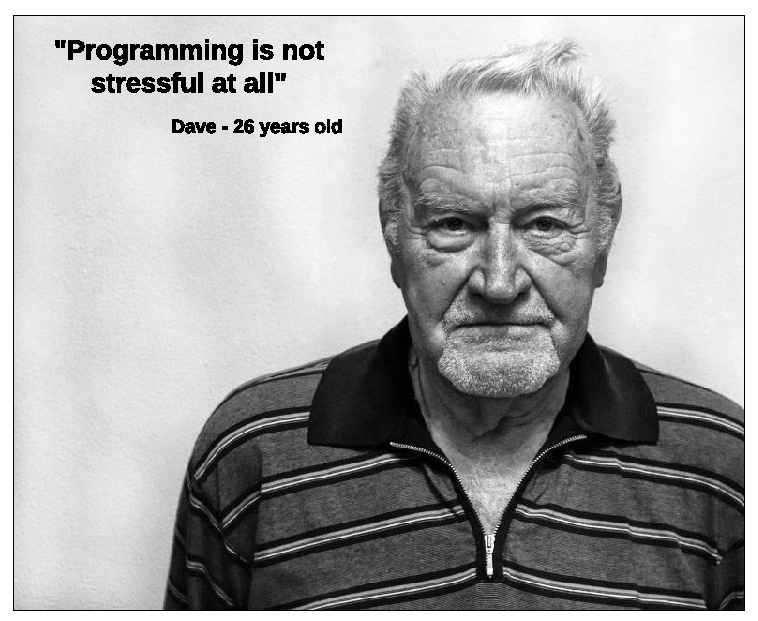
\includegraphics[width=10.5cm]{figures/lecture2/meme.pdf}
\end{figure}
    \end{center}
\vspace*{\fill}
\end{frame}


%=+=+=+=+=+=+=+=+=+=+=+=+=+=+=+=+=+=+=+=+=+=+=+=+=+=
\section{Programming Languages for ARIAC}
%=+=+=+=+=+=+=+=+=+=+=+=+=+=+=+=+=+=+=+=+=+=+=+=+=+=
\begin{frame}[fragile]{\sec}
\vspace*{\fill}

{\large \mynote Programming Languages in ARIAC} \doublerulefill


\begin{center} 
    \begin{compactitem}
    \item \CC and Python can be used to develop a control system for ARIAC.
    \item There is an \urllink{https://github.com/UniversalRobots/Universal_Robots_ROS2_Gazebo_Simulation/issues/19}{issue} with  UR robot controllers in ROS Humble.
    \item UR robot controllers work in ROS Galactic but the Python Moveit API is still being ported.
    \begin{compactitem}
    \item \textbf{Solution \#1}
        \begin{compactitem}
            \item Use only \CC
        \end{compactitem}
        \item \textbf{Solution \#2}
        \begin{compactitem}
            \item Use Python to interface with ARIAC to retrieve orders and to detect challenges.
            \item Use \CC to control the robot with Moveit.
        \end{compactitem}
    \end{compactitem}
    \end{compactitem}
    \end{center}
\vspace*{\fill}
\end{frame}


%=+=+=+=+=+=+=+=+=+=+=+=+=+=+=+=+=+=+=+=+=+=+=+=+=+=
\section{Linux Basics}
%=+=+=+=+=+=+=+=+=+=+=+=+=+=+=+=+=+=+=+=+=+=+=+=+=+=
\begin{frame}[fragile]{\sec}
\vspace*{\fill}
\begin{center} 
%%%%%%%%%%%%%%%%%%%%%%%%%%%%%%%%%%%%%%%%%%%%%%%%
{\large \mydefinition Shell} \doublerulefill

\emph{A program which takes keyboard commands and passes them to the OS to carry out.}

\begin{compactitem}
    \item The Bourne shell (\texttt{sh}), developed by Steve Bourne, is regarded as the first UNIX shell ever but it has many drawbacks. 
    \item Many shells were developed to improve the Bourne Shell.
    \begin{compactitem}
    \footnotesize
        \item The GNU Bourne-Again Shell (\texttt{bash}), the C Shell (\texttt{csh}), the Korn shell (\texttt{ksh}), the Z shell (\texttt{zsh}), etc.
        \item Check the current shell of your system with \myTerminal{ps -p \$\$} 
    \end{compactitem}
    \item A shell script is a plain text file which contains a series of shell commands. Anything you can run normally on the command line can be put into a script and vice-versa.
    \item \mynote I use \urllink{https://github.com/ohmyzsh/ohmyzsh/wiki/Installing-ZSH}{zsh} instead of bash.
\end{compactitem}

\end{center}
\vspace*{\fill}
\end{frame}


\begin{frame}[fragile]{\sec}
\vspace*{\fill}
\begin{center} 
%%%%%%%%%%%%%%%%%%%%%%%%%%%%%%%%%%%%%%%%%%%%%%%%
{\large \mydefinition Terminal} \doublerulefill

\emph{A text window program that runs a shell (BASH shell in Ubuntu).}
\begin{compactitem}
\small
        \item Some bash commands are blocking and the only way to terminate these commands is to click in the terminal and then \myKeyboardShortcut{Ctrl+c}
        \item You can open a terminal with \myKeyboardShortcut{Ctrl+Alt+t}
        \item \mynote I use \urllink{https://gnome-terminator.org/}{terminator} for the terminal.
        \item \mybestpractice Be efficient, use the \myKeyboardShortcut{Tab} key for auto-completion when working with the terminal.
    \end{compactitem}
\end{center}
\vspace*{\fill}
\end{frame}

% \begin{frame}[fragile]{\sec}
% \vspace*{\fill}
% \begin{center} 
% %%%%%%%%%%%%%%%%%%%%%%%%%%%%%%%%%%%%%%%%%%%%%%%%
% {\large \mynote} \doublerulefill


% \begin{compactitem}
%     \large
%     \item I use \urllink{https://github.com/ohmyzsh/ohmyzsh/wiki/Installing-ZSH}{zsh} instead of bash.
%     \item I use \urllink{https://gnome-terminator.org/}{terminator} for the terminal.

% \end{compactitem}
% \end{center}
% \vspace*{\fill}
% \end{frame}

%=+=+=+=+=+=+=+=+=+=+=+=+=+=+=+=+=+=+=+=+=+=+=+=+=+=
% \begin{frame}[fragile]{\sec}
% \vspace*{\fill}
% \begin{center} 

% {\Large \mybestpractice} \doublerulefill

% {\large Be efficient, use the \mykbNormal{Tab} key for autocompletion when working with the terminal.}
% \end{center}
% \vspace*{\fill}
% \end{frame}

%=+=+=+=+=+=+=+=+=+=+=+=+=+=+=+=+=+=+=+=+=+=+=+=+=+=
\subsection{bashrc}
%=+=+=+=+=+=+=+=+=+=+=+=+=+=+=+=+=+=+=+=+=+=+=+=+=+=
\begin{frame}[fragile]{\secsec}
\vspace*{\fill}
\begin{center} 

{\large \mydefinition bashrc File} \doublerulefill

\myFile{bashrc} \emph{ is a hidden bash script located in your home directory and runs whenever it is started interactively. It initializes an interactive shell session. In other words, everything in this script is executed when you open a terminal.}

\hrulefill


\begin{compactitem}
    \item \myFile{bashrc} is a hidden file located in your Home directory.
    \item To display hidden files and folders:
    \begin{compactitem}
        \item \myTerminal{ls -a} in a terminal.
        \item From a GUI file manager: \myKeyboardShortcut{Ctrl+h}
    \end{compactitem}
    \item You put commands in this file to set up the shell for use in your particular environment, or to customize things to your preferences.
    \begin{compactitem}
        \item Common things to put in \myFile{bashrc} are functions, aliases, and environment variables.
    \end{compactitem}
\end{compactitem}
\end{center}
\vspace*{\fill}
\end{frame}


%=+=+=+=+=+=+=+=+=+=+=+=+=+=+=+=+=+=+=+=+=+=+=+=+=+=
\subsubsection*{Functions}
%=+=+=+=+=+=+=+=+=+=+=+=+=+=+=+=+=+=+=+=+=+=+=+=+=+=
\begin{frame}[fragile]{\secsecsec}
\vspace*{\fill}
\begin{center} 

{\large \mycodesyntax Functions} \doublerulefill

Bash functions may be declared in two different formats.

\begin{columns}[T]
    \begin{column}{0.5\textwidth}

\begin{compactitem}
    \begin{bashscriptsyntax}
function_name () {
  commands
}
\end{bashscriptsyntax}
\item Example:
\begin{bashscript}
greeting () {
  echo Hello
}
\end{bashscript}

\myTerminal{greeting} to call the function.
\end{compactitem}
    \end{column}
    
\begin{column}{0.5\textwidth}
\begin{compactitem}
    \begin{bashscriptsyntax}
function function_name {
  commands
}
\end{bashscriptsyntax}
\item Example:
\begin{bashscript}
function greeting () {
  echo Hello
}
\end{bashscript}

\myTerminal{greeting} to call the function.
\end{compactitem}
\end{column}
 \end{columns}
%%%%%%%%%%%%%%%%%%%%%%%%%%%%%%%%%%%%%%%%%%%%%%%%
\end{center}
\vspace*{\fill}
\end{frame}


%=+=+=+=+=+=+=+=+=+=+=+=+=+=+=+=+=+=+=+=+=+=+=+=+=+=
\begin{frame}[fragile]{\secsecsec}
\vspace*{\fill}
\begin{center} 

{\large \mycodesyntax Functions} \doublerulefill

Passing arguments to a function.


\begin{compactitem}

\begin{bashscript}
greeting () {
  echo Hello $1 $2
}
\end{bashscript}

\myTerminal{greeting John Doe} to call the function with arguments.
\item The parameters are \$1, \$2, \ldots, corresponding to the position of the argument passed after the function's name.
\item The \$0 variable is reserved for the function's name.
\item The \$\#  variable holds the number of positional parameters/arguments passed to the function.
\begin{bashscript}
test(){                
    echo $0 $# $1 $2
}

\end{bashscript}

\myTerminal{test a b c d e f}
\end{compactitem}
%%%%%%%%%%%%%%%%%%%%%%%%%%%%%%%%%%%%%%%%%%%%%%%%

\end{center}
\vspace*{\fill}
\end{frame}



%=+=+=+=+=+=+=+=+=+=+=+=+=+=+=+=+=+=+=+=+=+=+=+=+=+=
\subsubsection*{Aliases}
%=+=+=+=+=+=+=+=+=+=+=+=+=+=+=+=+=+=+=+=+=+=+=+=+=+=
\begin{frame}[fragile]{\secsecsec}
\vspace*{\fill}
\begin{center} 

{\large \mydefinition Aliases} \doublerulefill

\emph{Bash aliases are essentially shortcuts that can save you from having to remember or type long commands.}


\begin{compactitem}
\item The syntax to create an alias:
\begin{bashscriptsyntax}
alias identifier="value"
\end{bashscriptsyntax}
\begin{compactitem}
    \item An alias declaration starts with the \bashFootnote{alias} keyword followed by the alias identifier, an equal sign and the value (the command you want to run for the alias). 
        \item The command needs to be enclosed in quotes and with \emph{no spacing around the equal sign}. 
        \item Each alias needs to be declared on a new line.
        \item Aliases can be declared anywhere in the file.
\end{compactitem}
\item Aliases I will be using in ROS lectures:
    \begin{bashscript}
    alias ..="cd .."
    alias sr="source /home/zeid/.zshrc"
    # alias sr="source /home/zeid/.bashrc"
    \end{bashscript}
\item \mynote New aliases will be created when needed.
\end{compactitem}


\end{center}
\vspace*{\fill}
\end{frame}


%=+=+=+=+=+=+=+=+=+=+=+=+=+=+=+=+=+=+=+=+=+=+=+=+=+=
\subsection{source}
\begin{frame}[fragile]{\secsec}
\vspace*{\fill}
\begin{center} 

{\large \mynote source Command} \doublerulefill


If you modify \myFile{bashrc} with a terminal already opened, your modifications will not automatically take effect in the current terminal.


\myhrulefill

\begin{compactitem}
% \item Opening a new terminal each time is not efficient at all.
\item The command \myTool{source <file>} allows you to execute each line of a file in the current terminal.
\item To reload \myFile{bashrc} in the current terminal: \myTerminal{source \textasciitilde/.bashrc} (or create an alias for this command as seen in the previous slide).
\item \mynote The command \myTool{. <file>} does the same thing as \myTool{source <file>}
\end{compactitem}

\end{center}
\vspace*{\fill}
\end{frame}


%=+=+=+=+=+=+=+=+=+=+=+=+=+=+=+=+=+=+=+=+=+=+=+=+=+=
\section{Robot Operating System (ROS)}
\begin{frame}[fragile]{\sec}
\vspace*{\fill}
\begin{center} 

{\large \mydefinition} \doublerulefill

{\emph{ROS is not really an operating system (OS) but more like a software development kit (SDK). According to Brian Gerkey\footnote{\tiny{\url{https://answers.ros.org/question/12230/what-is-ros-exactly-middleware-framework-operating-system/}}}, ROS is a combination of plumbing, tools, capabilities, and ecosystem.}}


\includegraphics[width=13cm]{figures/lecture2/ros-equation.png}

\begin{compactitem}
\footnotesize
\item Prototypes originated from Standford AI research and officially released by Willow Garage in 2017.
    \item ROS is currently maintained by \urllink{https://www.openrobotics.org/}{Open Robotics}.
    \item \mytodo Watch the video on \urllink{https://ros.org/}{https://ros.org/}
\end{compactitem}
\end{center}
\vspace*{\fill}
\end{frame}


%=+=+=+=+=+=+=+=+=+=+=+=+=+=+=+=+=+=+=+=+=+=+=+=+=+=
\subsection{Resource}
%=+=+=+=+=+=+=+=+=+=+=+=+=+=+=+=+=+=+=+=+=+=+=+=+=+=
\begin{frame}[fragile]{\secsec}
\vspace*{\fill}
\begin{center} 

{\large \mynote Resources} \doublerulefill

\begin{compactitem}
    \item Official website: \urllink{http://wiki.ros.org/}{http://wiki.ros.org/}
    \item Tutorials: \urllink{http://wiki.ros.org/ROS/Tutorials}{http://wiki.ros.org/ROS/Tutorials}
    \item ROS index: \urllink{https://index.ros.org/packages/#galactic}{https://index.ros.org/packages/#galactic}
    \item ROS discourse: \urllink{https://discourse.ros.org/}{https://discourse.ros.org/}
    \item REPs: \urllink{https://www.ros.org/reps/rep-0001.html}{https://www.ros.org/reps/rep-0001.html}
\end{compactitem}
\end{center}
\vspace*{\fill}
\end{frame}

%=+=+=+=+=+=+=+=+=+=+=+=+=+=+=+=+=+=+=+=+=+=+=+=+=+=
\subsection{Why ROS2?}
%=+=+=+=+=+=+=+=+=+=+=+=+=+=+=+=+=+=+=+=+=+=+=+=+=+=
\begin{frame}[fragile]{\secsec}
\vspace*{\fill}
\begin{center} 

{\large \mynote ROS1: Drawbacks} \doublerulefill

\begin{compactitem}
    \item ROS1 was mainly developed for the academic research community in 2007 by Willow Garage.
    \item Over the years, ROS1 has become huge in the open source robotic communities.
    \item Companies and agencies can not use ROS1 due to lack of  important requirements.
    \begin{compactitem}
        \item No \emph{real time}: The purpose of ROS1 was to save development time and not to ensure real-time operations.
        \item No \emph{security} because modules communicate over standard networking protocols, which are prone to cyber attacks.
        \item No \emph{safety certification} means it can not ensure the safety of people using it.
    \end{compactitem}
    \item While ROS1 is holding up well, to better meet the needs of a now-broader ROS community, new use cases must be addressed.
\end{compactitem}
\end{center}
\vspace*{\fill}
\end{frame}

%=+=+=+=+=+=+=+=+=+=+=+=+=+=+=+=+=+=+=+=+=+=+=+=+=+=
\begin{frame}[fragile]{\secsec}
\vspace*{\fill}
\begin{center} 
{\large \mynote ROS1: Missing Use Cases} \doublerulefill


   \begin{compactitem}
   \item \emph{Teams of multiple robots}: No standard approach to build multi-robot systems. They are all somewhat of a hack on top of the single-master structure (no multi masters concept).
   \item \emph{Small embedded platforms}: ROS1 does not allow small computers, including micro controllers, to be first-class participants in the ROS environment.
   \item \emph{Non-ideal networks}: ROS1 does not behave well when network connectivity degrades due to loss and/or delay, from poor-quality WiFi to ground-to-space communication links.
   \end{compactitem}

\end{center}
\vspace*{\fill}
\end{frame}

%=+=+=+=+=+=+=+=+=+=+=+=+=+=+=+=+=+=+=+=+=+=+=+=+=+=
\subsection{ROS2}
%=+=+=+=+=+=+=+=+=+=+=+=+=+=+=+=+=+=+=+=+=+=+=+=+=+=
\begin{frame}[fragile]{\secsec}
\vspace*{\fill}
\begin{center} 
{\large \mynote ROS2: Overview} \doublerulefill

\begin{itemize}
    \item ROS2 is not built on top of ROS1. ROS developers wanted ROS1 as it exists today to keep working and be unaffected by the development of ROS2. \item The API in ROS2 has been modified since most of the code in ROS1 is from 2007-2009.
   \item The key concepts (e.g., Nodes, Topics, Messages) still remain the same in ROS2 but by default, ROS2 API-code is not compatible with existing ROS1 code.
   \begin{itemize}
       \item ROS1 code can still be run in ROS2 with a bridge from ROS1 to ROS2 (see \urllink{https://github.com/ros2/ros1_bridge}{ros1_bridge}).
   \end{itemize}
   \item Some packages from ROS1 are still being ported to ROS2.
   \end{itemize}
\end{center}
\vspace*{\fill}
\end{frame}

%=+=+=+=+=+=+=+=+=+=+=+=+=+=+=+=+=+=+=+=+=+=+=+=+=+=
\begin{frame}[fragile]{\secsec}
\vspace*{\fill}
\begin{center} 
    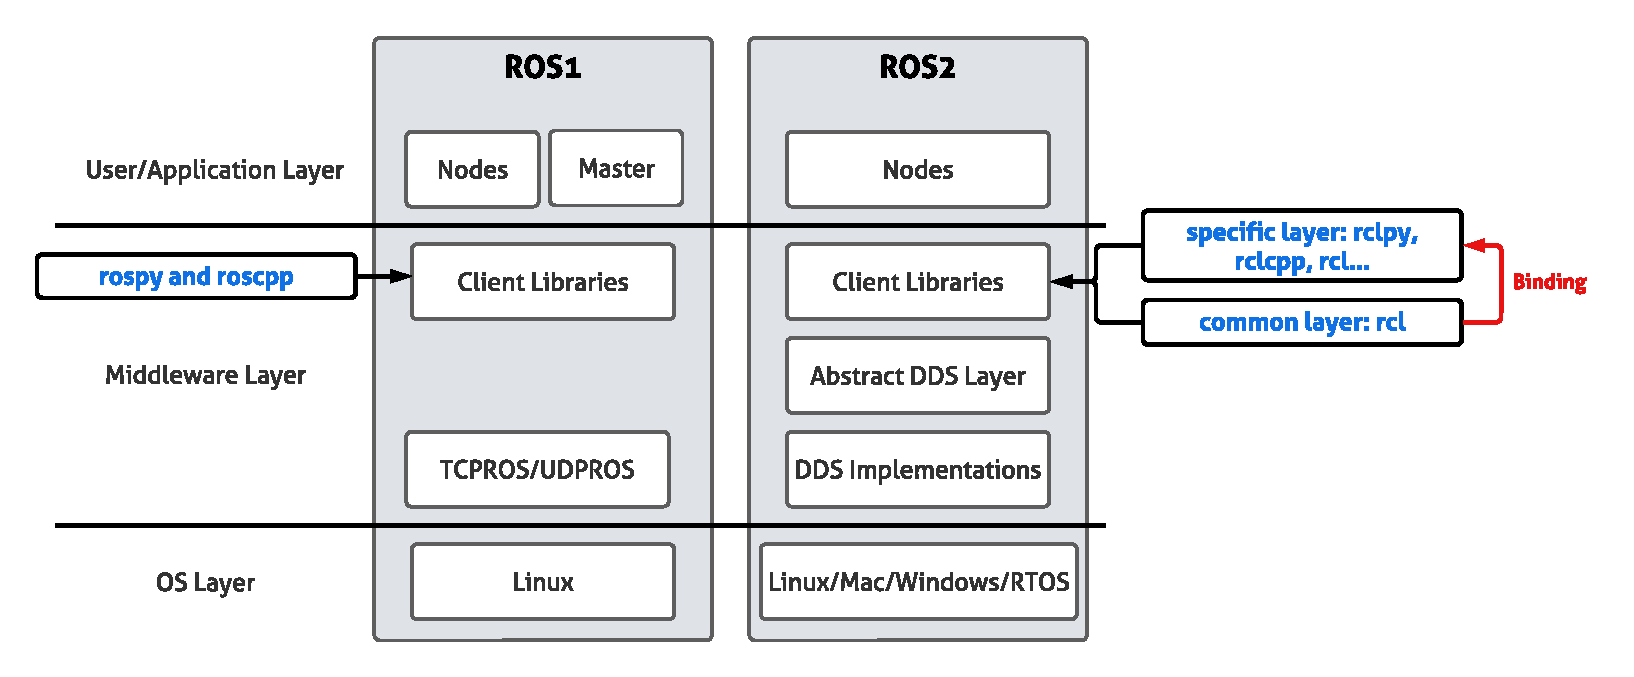
\includegraphics[width=15cm]{figures/lecture2/ros1_ros2_architecture.pdf}
\end{center}
\vspace*{\fill}
\end{frame}

%=+=+=+=+=+=+=+=+=+=+=+=+=+=+=+=+=+=+=+=+=+=+=+=+=+=
\subsubsection*{DDS}
%=+=+=+=+=+=+=+=+=+=+=+=+=+=+=+=+=+=+=+=+=+=+=+=+=+=
\begin{frame}[fragile]{\secsecsec}
\vspace*{\fill}
\begin{center} 

{\large \mynote DDS: Data Distributed Service} \doublerulefill


\begin{itemize}
\small
% \item When exploring options for the next generation communication system of ROS, Open Robotics initially considered to either improve the ROS1 transport or build a new middleware using component libraries. ROS developers finally decided to leverage an existing and well developed implementation of DDS. 
    \item DDS is a middleware which aims to enable high-performance data exchanges using a publish-subscribe transport (similar to ROS1 publish-subscribe transport).
    
    \item DDS  is a proven industry standard and it is implemented by many vendors: eProsima's Fast DDS, RTI's Connext DDS, Eclipse Cyclone DDS, and GurumNetworks GurumDDS.
    \item The DDS market is more general: Battleships, large utility installations like dams, financial systems, space systems, flight systems, train switchboard systems, and many more.

    \item The default discovery system provided by DDS is a distributed discovery system. This allows any two DDS Nodes to communicate without the need for the ROS Master. This makes the system more fault tolerant and flexible. 
    
\end{itemize}
\end{center}
\vspace*{\fill}
\end{frame}

%=+=+=+=+=+=+=+=+=+=+=+=+=+=+=+=+=+=+=+=+=+=+=+=+=+=
\begin{frame}[fragile]{\secsecsec}
%=+=+=+=+=+=+=+=+=+=+=+=+=+=+=+=+=+=+=+=+=+=+=+=+=+=
\vspace*{\fill}
\begin{center} 
{\large \mytodo Check DDS Version} \doublerulefill

\begin{enumerate}
\small
    \item \myTerminal{source /opt/ros/galactic/setup.bash}
    \item \myTerminal{ros2 doctor -{}-report}
\end{enumerate}

\hrulefill

\mynote If you want to use a different version of DDS implementation you need to \urllink{https://docs.ros.org/en/galactic/Installation/DDS-Implementations.html#}{install new packages}.
\end{center}
\vspace*{\fill}
\end{frame}

% %=+=+=+=+=+=+=+=+=+=+=+=+=+=+=+=+=+=+=+=+=+=+=+=+=+=
% \subsubsection*{Packages}
% %=+=+=+=+=+=+=+=+=+=+=+=+=+=+=+=+=+=+=+=+=+=+=+=+=+=
% \begin{frame}[fragile]{\secsecsec}
% %=+=+=+=+=+=+=+=+=+=+=+=+=+=+=+=+=+=+=+=+=+=+=+=+=+=
% \vspace*{\fill}
% \begin{center} 
% {\large \mytodo \textsc{Debian Packages}} \doublerulefill

% \begin{itemize}
%     \item ROS Debian packages (installed via \myterminalSmall{sudo apt install}) are located in  \mydirSmall{/opt/ros/galactic/share}
%     \begin{itemize}
%         \item \mywarning Never modify anything in this folder.
%         \item If you need to modify files from this folder, clone the package in your ROS workspace or copy/paste files in your ROS workspace.
%     \end{itemize}
% \end{itemize}
% \end{center}
% \vspace*{\fill}
% \end{frame}


%=+=+=+=+=+=+=+=+=+=+=+=+=+=+=+=+=+=+=+=+=+=+=+=+=+=
\subsubsection*{Colcon}
%=+=+=+=+=+=+=+=+=+=+=+=+=+=+=+=+=+=+=+=+=+=+=+=+=+=
\begin{frame}[fragile]{\secsecsec}
%=+=+=+=+=+=+=+=+=+=+=+=+=+=+=+=+=+=+=+=+=+=+=+=+=+=
\vspace*{\fill}
\begin{center} 

{\large \mytodo Install Extensions for VS Code} \doublerulefill

    \begin{compactitem}
        \item \urllink{https://marketplace.visualstudio.com/items?itemName=ms-iot.vscode-ros}{ROS}
        \item \urllink{https://marketplace.visualstudio.com/items?itemName=twxs.cmake}{CMake}
    \end{compactitem}


{\large \mytodo Install Colcon} \doublerulefill

\emph{\urllink{https://colcon.readthedocs.io/en/released/}{colcon} is a command line tool to improve the workflow of building, testing and using multiple software packages.}


\begin{compactitem}
    \item Install colcon:
    \begin{compactitem}
        \item \myTerminal{sudo apt update}
        \item \myTerminal{sudo apt install python3-colcon-common-extensions}
    \end{compactitem}
\end{compactitem}
\end{center}
\vspace*{\fill}
\end{frame}

% %=+=+=+=+=+=+=+=+=+=+=+=+=+=+=+=+=+=+=+=+=+=+=+=+=+=
% \subsubsection*{Setup .bashrc}
% %=+=+=+=+=+=+=+=+=+=+=+=+=+=+=+=+=+=+=+=+=+=+=+=+=+=
% \begin{frame}[fragile]{\secsecsec}
% %=+=+=+=+=+=+=+=+=+=+=+=+=+=+=+=+=+=+=+=+=+=+=+=+=+=
% \vspace*{\fill}
% \begin{center} 
% {\large \mytodo Set up the Linux environment for ROS2} \doublerulefill


% \begin{compactitem}
%     \item Edit \myfileFoot{.bashrc}
%     \begin{compactitem}
%         \item \bashFootnote{source /opt/ros/galactic/setup.bash}
%         \item \bashFootnote{source /usr/share/colcon_argcomplete/hook/colcon-argcomplete.bash}
%         \item \bashFootnote{source /usr/share/colcon_cd/function/colcon_cd.sh}
%         \item \bashFootnote{eval "$(register-python-argcomplete3 ros2)"}
%         \item \bashFootnote{eval "$(register-python-argcomplete3 colcon)"}
%     \end{compactitem}
% \end{compactitem}
% \end{center}
% \vspace*{\fill}
% \end{frame}


%=+=+=+=+=+=+=+=+=+=+=+=+=+=+=+=+=+=+=+=+=+=+=+=+=+=
\subsubsection*{Setup .bashrc or .zshrc}
%=+=+=+=+=+=+=+=+=+=+=+=+=+=+=+=+=+=+=+=+=+=+=+=+=+=
\begin{frame}[fragile]{\secsecsec}
%=+=+=+=+=+=+=+=+=+=+=+=+=+=+=+=+=+=+=+=+=+=+=+=+=+=
\vspace*{\fill}
\begin{center} 
{\large \mytodo Set up the Linux environment for ROS2} \doublerulefill

\begin{compactitem}
\footnotesize
\item Edit \myfileFoot{.bashrc}
    \begin{bashScriptList}
source /opt/ros/galactic/setup.bash
source /usr/share/colcon_argcomplete/hook/colcon-argcomplete.bash
source /usr/share/colcon_cd/function/colcon_cd.sh
eval "$(register-python-argcomplete3 ros2)"
eval "$(register-python-argcomplete3 colcon)"
    \end{bashScriptList}

\item Edit \myfileFoot{.zshrc}
    \begin{bashScriptList}
source /opt/ros/galactic/setup.zsh
source /usr/share/colcon_argcomplete/hook/colcon-argcomplete.zsh
source /usr/share/colcon_cd/function/colcon_cd.sh
eval "$(register-python-argcomplete3 ros2)"
eval "$(register-python-argcomplete3 colcon)"
    \end{bashScriptList}
    
\end{compactitem}
\end{center}
\vspace*{\fill}
\end{frame}

%=+=+=+=+=+=+=+=+=+=+=+=+=+=+=+=+=+=+=+=+=+=+=+=+=+=
\section{Node, Topic, and Message}
%=+=+=+=+=+=+=+=+=+=+=+=+=+=+=+=+=+=+=+=+=+=+=+=+=+=
\begin{frame}[fragile]{\sec}
\vspace*{\fill}

%%%%%%%%%%%%%%%%%%%%%%%%%%%%%%%%%%%%%%%%%%%%%%%%

{\large \mydefinition Node} \doublerulefill

\large \emph{A \urllink{http://wiki.ros.org/ROS/Tutorials/UnderstandingNodes}{Node} is a small program written in Python or \CC that executes some relatively simple task or process. Nodes are usually categorized into Publishers (send data) and Subscribers (receive data).} 


{\large \mydefinition Topic} \doublerulefill

\large \emph{A \urllink{http://wiki.ros.org/Topics}{Topic} is a named bus\footnote{A communication system that transfers data between components inside a computer or between computers} over which Nodes exchange Messages.}

{\large \mydefinition Message} \doublerulefill

\large \emph{A \urllink{http://wiki.ros.org/Messages}{Message} is a packet of data (a simple data structure comprising typed fields).}

\vspace*{\fill}
\end{frame}

%=+=+=+=+=+=+=+=+=+=+=+=+=+=+=+=+=+=+=+=+=+=+=+=+=+=
\begin{frame}[fragile]{\sec}
\vspace*{\fill}
\begin{center} 
Analogy from \urllink{https://www.skillshare.com/profile/Edouard-Renard/690578289}{Edouard Renard}.

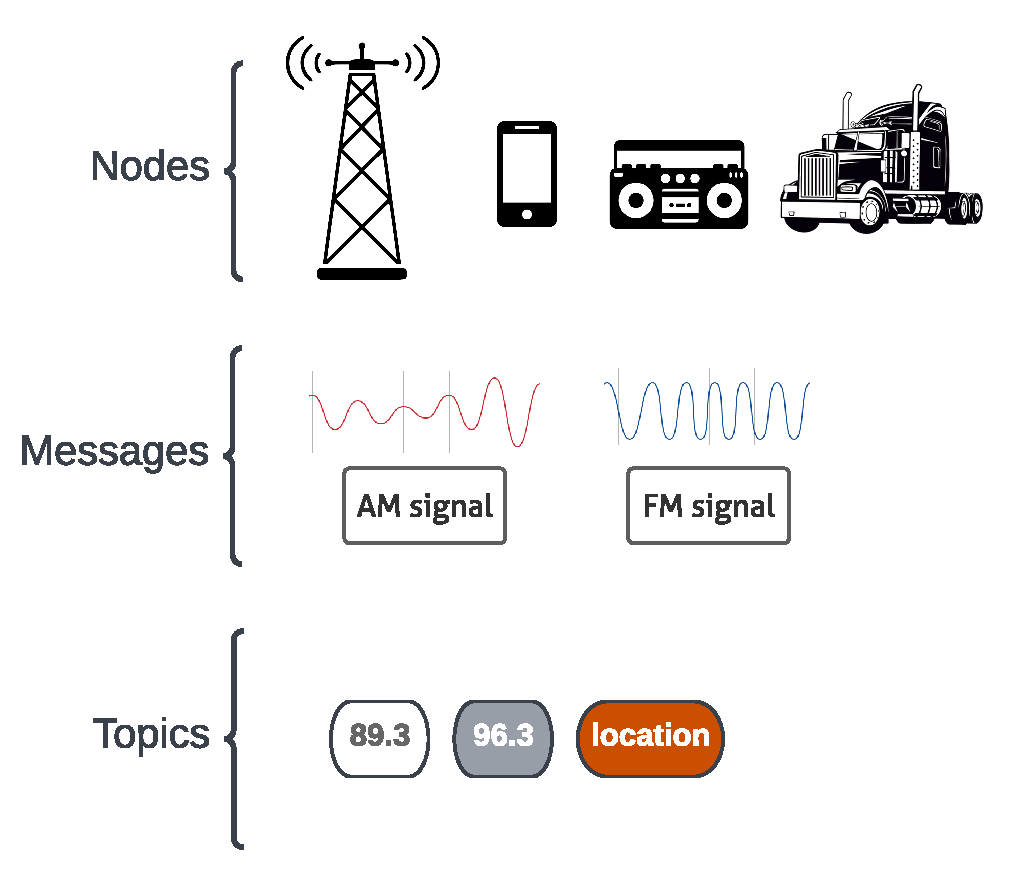
\includegraphics[width=.6\linewidth]{figures/lecture2/analogy1.pdf}

\end{center}
\vspace*{\fill}
\end{frame}

%=+=+=+=+=+=+=+=+=+=+=+=+=+=+=+=+=+=+=+=+=+=+=+=+=+=
\begin{frame}[fragile]{\sec}
\vspace*{\fill}
\begin{center} 
Publishers and subscribers must work with the same Message type.

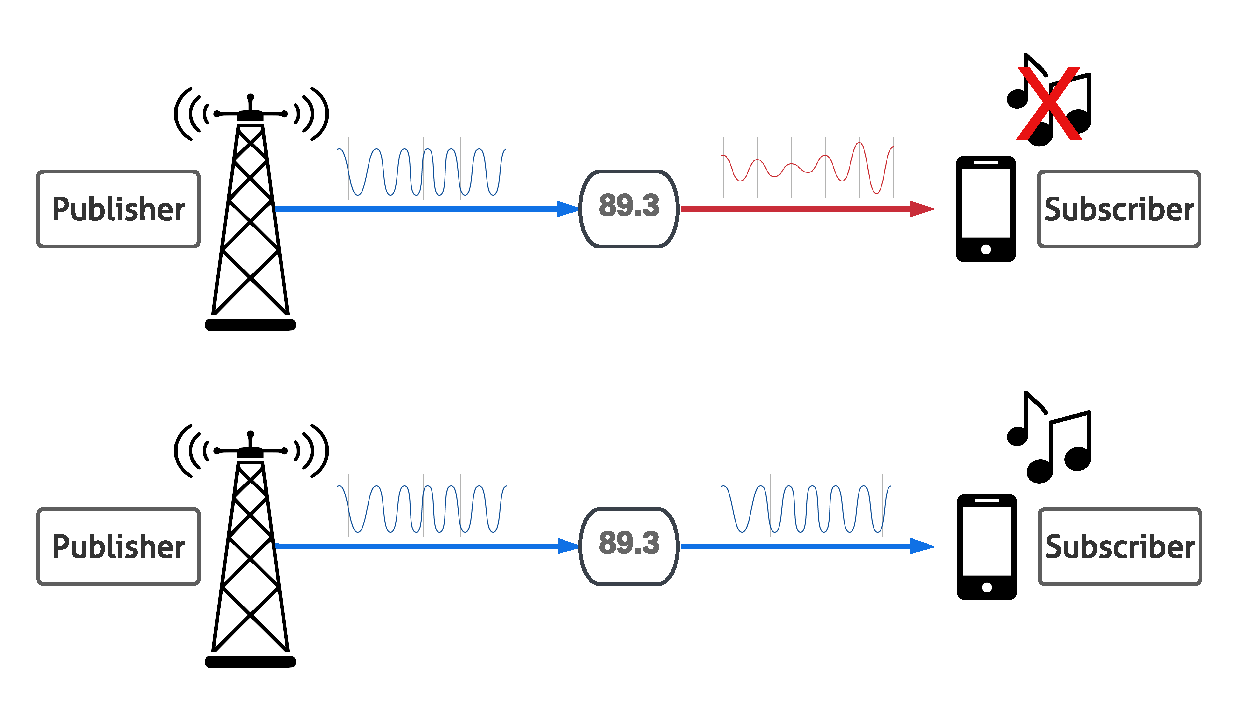
\includegraphics[width=.7\linewidth]{figures/lecture2/analogy2.pdf}

\end{center}
\vspace*{\fill}
\end{frame}


%=+=+=+=+=+=+=+=+=+=+=+=+=+=+=+=+=+=+=+=+=+=+=+=+=+=
\begin{frame}[fragile]{\sec}
\vspace*{\fill}
\begin{center} 
Publishers and subscribers must work with the same Topic name.

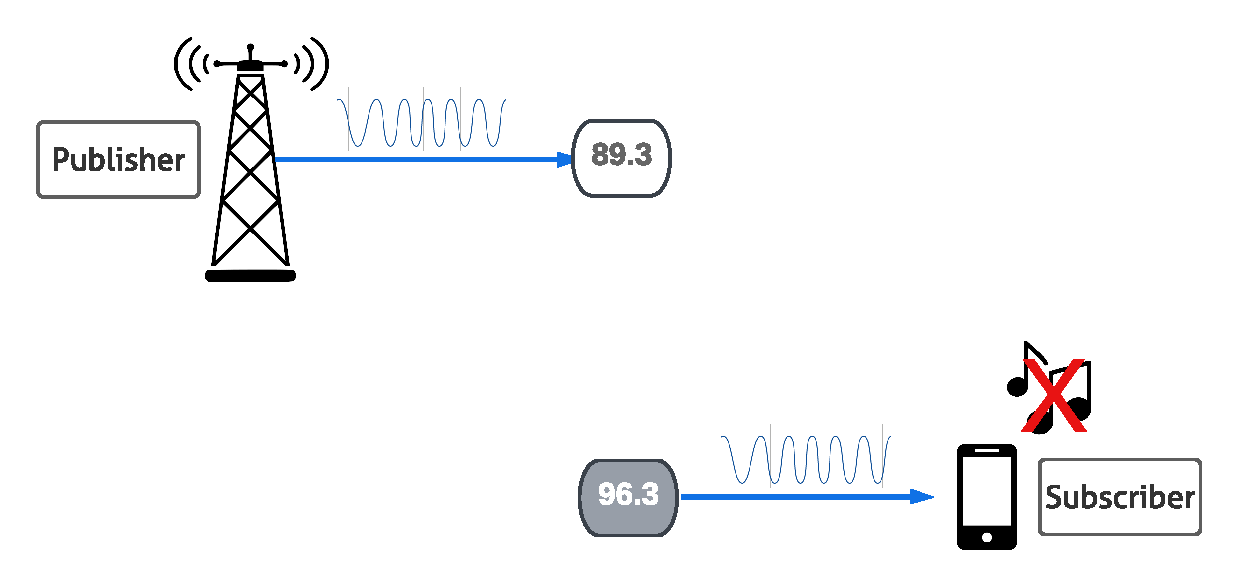
\includegraphics[width=.7\linewidth]{figures/lecture2/analogy3.pdf}

\end{center}
\vspace*{\fill}
\end{frame}


%=+=+=+=+=+=+=+=+=+=+=+=+=+=+=+=+=+=+=+=+=+=+=+=+=+=
\begin{frame}[fragile]{\sec}
\vspace*{\fill}
\begin{center} 
The goal of Publishers is to only send Messages to Topics.

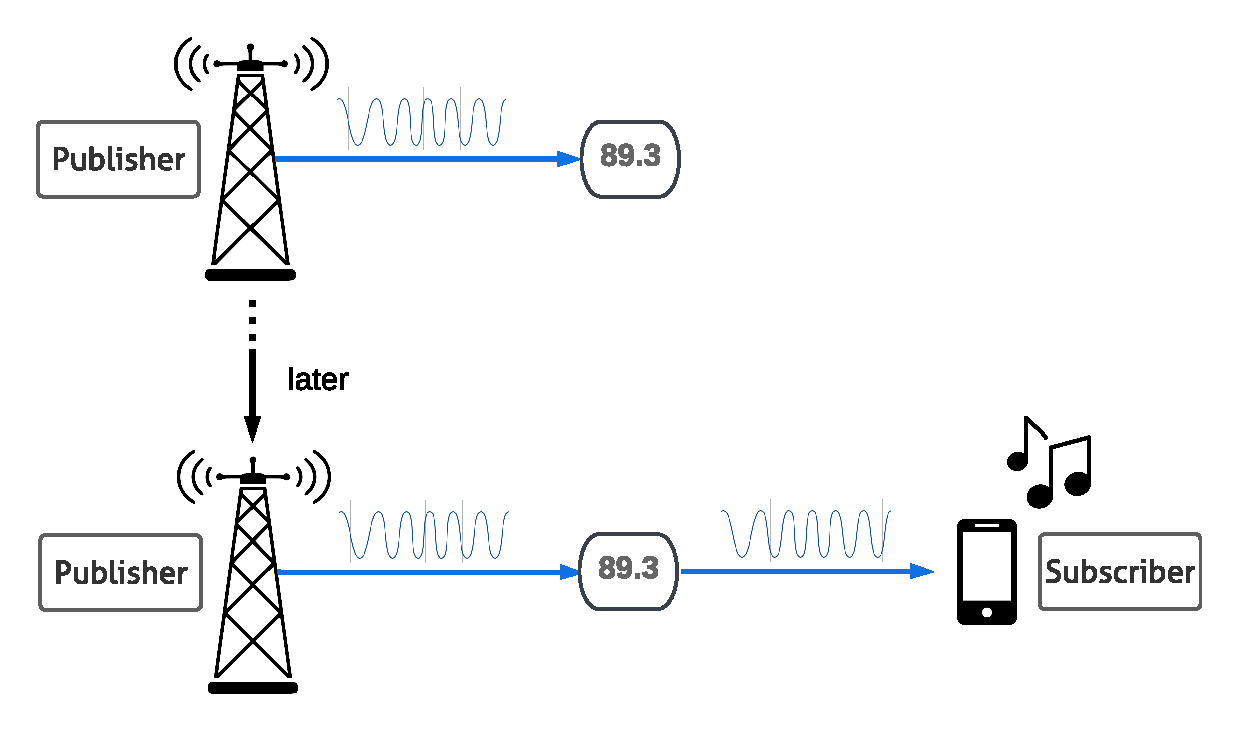
\includegraphics[width=.7\linewidth]{figures/lecture2/analogy4.pdf}

\end{center}
\vspace*{\fill}
\end{frame}


%=+=+=+=+=+=+=+=+=+=+=+=+=+=+=+=+=+=+=+=+=+=+=+=+=+=
\begin{frame}[fragile]{\sec}
\vspace*{\fill}
\begin{center} 
The goal of Subscribers is to only receive Messages from Topics.

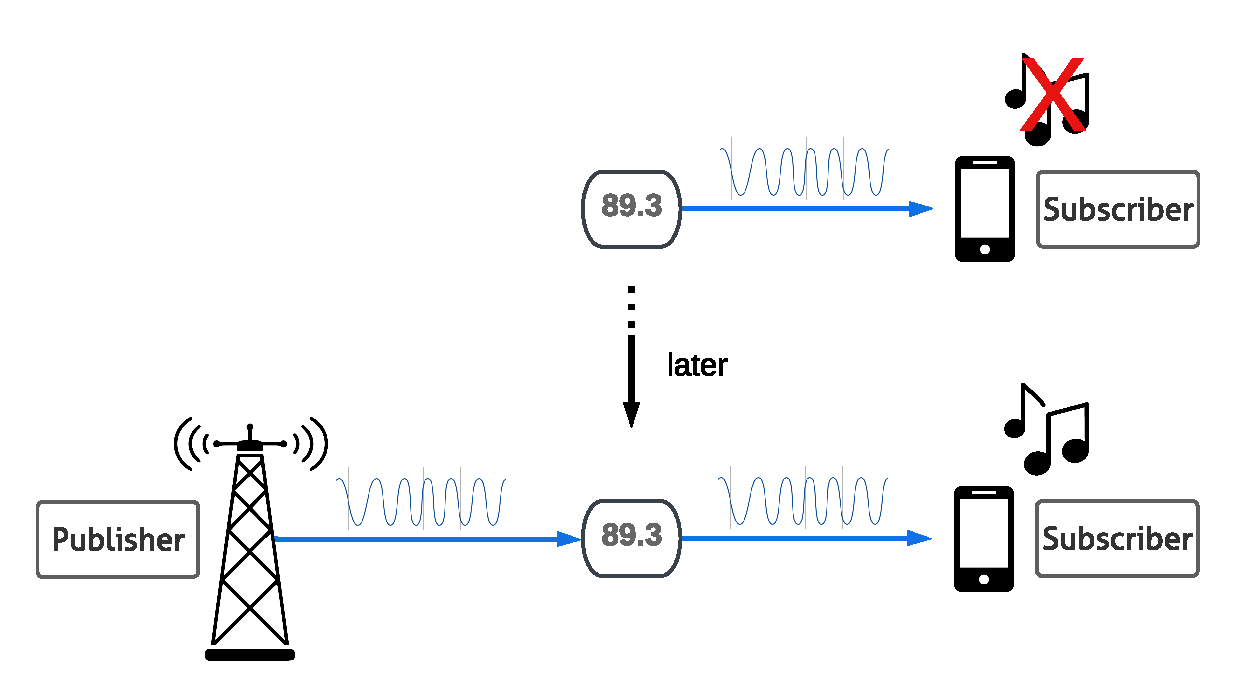
\includegraphics[width=.7\linewidth]{figures/lecture2/analogy5.pdf}

\end{center}
\vspace*{\fill}
\end{frame}



%=+=+=+=+=+=+=+=+=+=+=+=+=+=+=+=+=+=+=+=+=+=+=+=+=+=
\begin{frame}[fragile]{\sec}
\vspace*{\fill}
\begin{center} 
There can be multiple Subscribers to a Topic. 

\begin{compactitem}
\footnotesize
\item Publishers are not aware who is receiving the Messages. Their goal is to send Messages.
\item Subscribers are not aware who is sending the Messages. Their goal is to receive the Messages.
\end{compactitem}

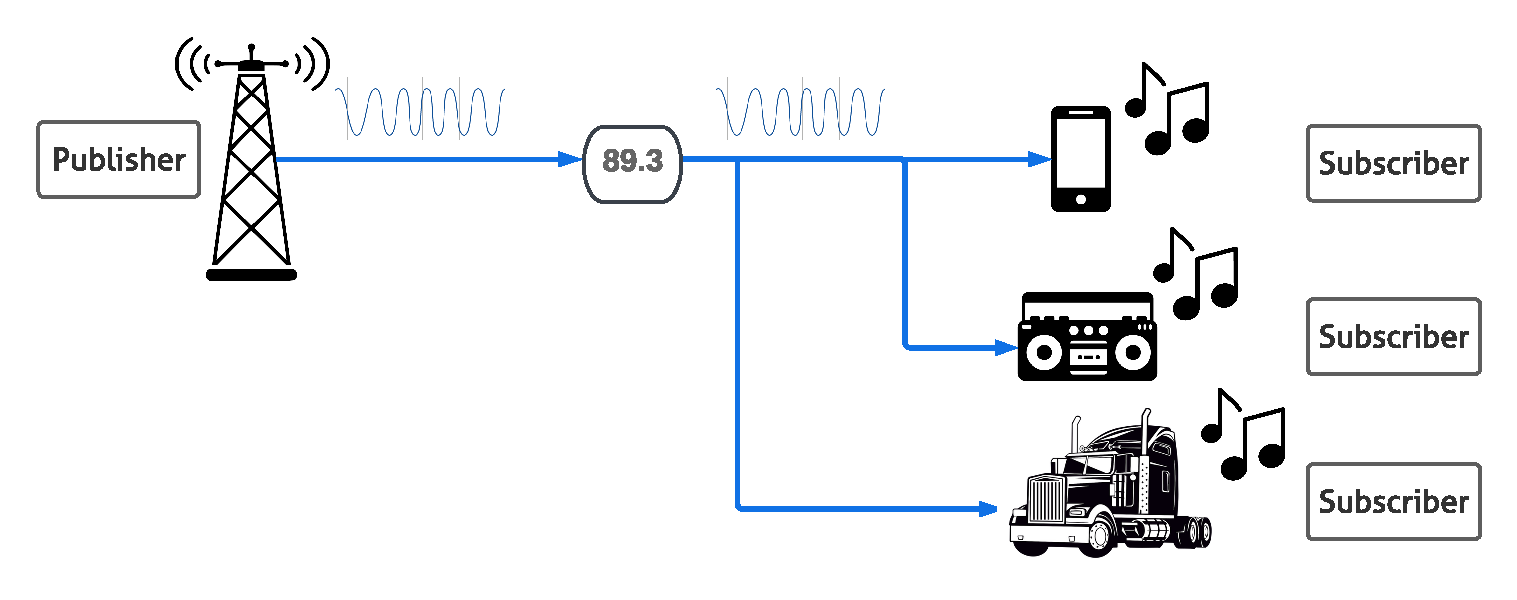
\includegraphics[width=.7\linewidth]{figures/lecture2/analogy6.pdf}

\end{center}
\vspace*{\fill}
\end{frame}

 
%=+=+=+=+=+=+=+=+=+=+=+=+=+=+=+=+=+=+=+=+=+=+=+=+=+=
\begin{frame}[fragile]{\sec}
\vspace*{\fill}
\begin{center} 
There can be multiple Publishers to the same Topic. 

\begin{compactitem}
\footnotesize

\item In this analogy, multiple radio stations can send signals to the same radio frequency. You may listen to a Pop music channel in Maryland but to a Country music channel in Texas.
\item \mynote In ROS, a Topic remapping is performed.
\end{compactitem}

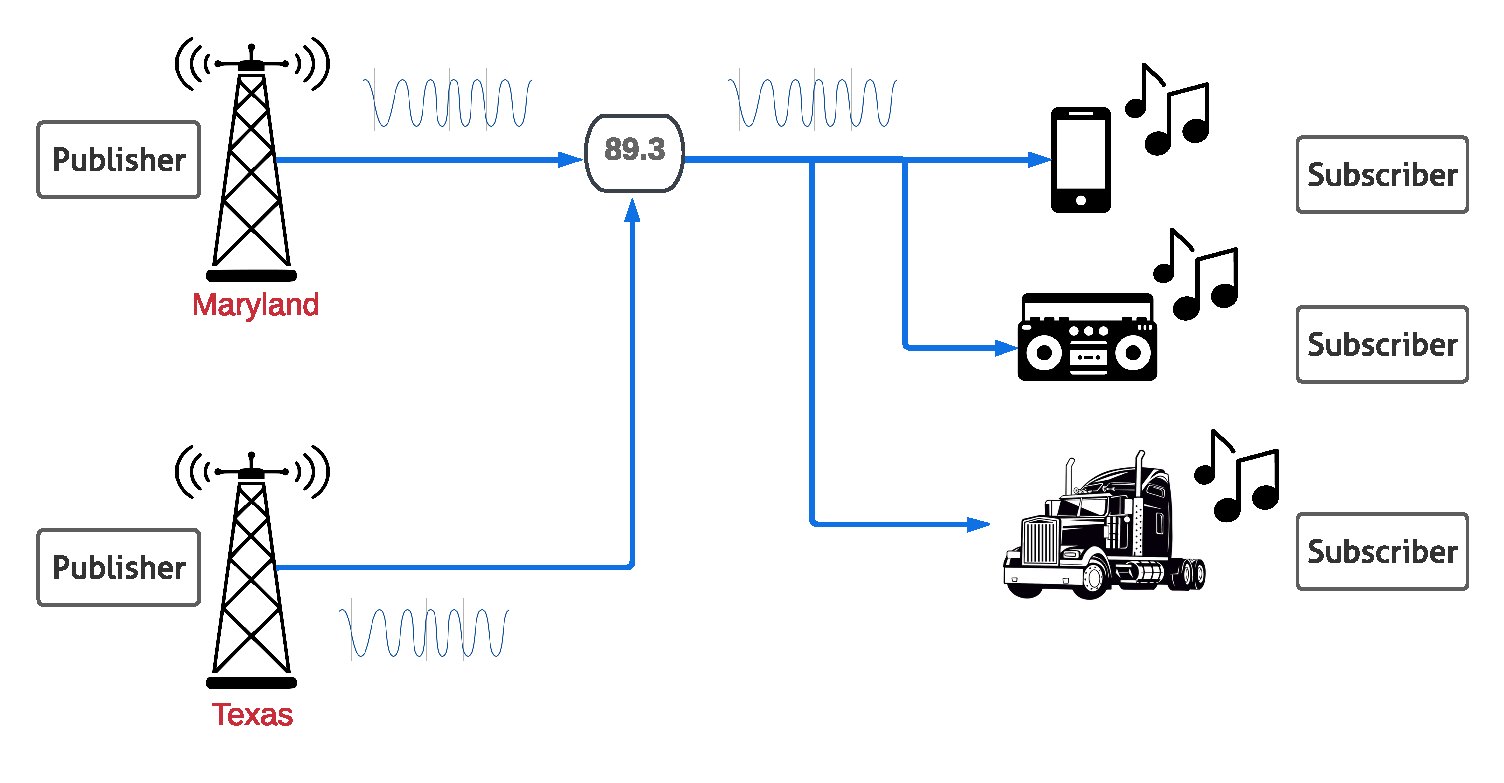
\includegraphics[width=.7\linewidth]{figures/lecture2/analogy7.pdf}

\end{center}
\vspace*{\fill}
\end{frame}


%=+=+=+=+=+=+=+=+=+=+=+=+=+=+=+=+=+=+=+=+=+=+=+=+=+=
\begin{frame}[fragile]{\sec}
\vspace*{\fill}
\begin{center} 
A Publisher can publish to different Topics.

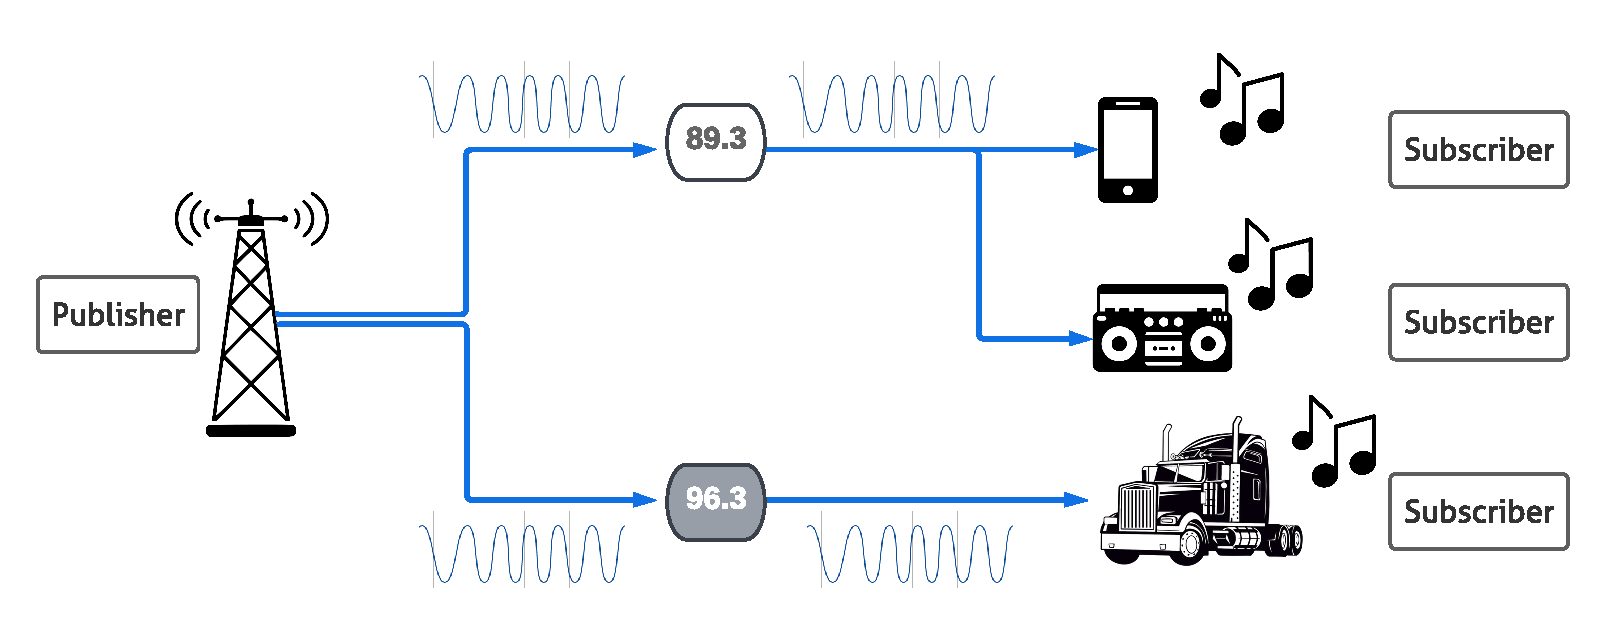
\includegraphics[width=.8\linewidth]{figures/lecture2/analogy8.pdf}

\end{center}
\vspace*{\fill}
\end{frame}



%=+=+=+=+=+=+=+=+=+=+=+=+=+=+=+=+=+=+=+=+=+=+=+=+=+=
\begin{frame}[fragile]{\sec}
\vspace*{\fill}
\begin{center} 
A Node can be both a Publisher and a Subscriber.

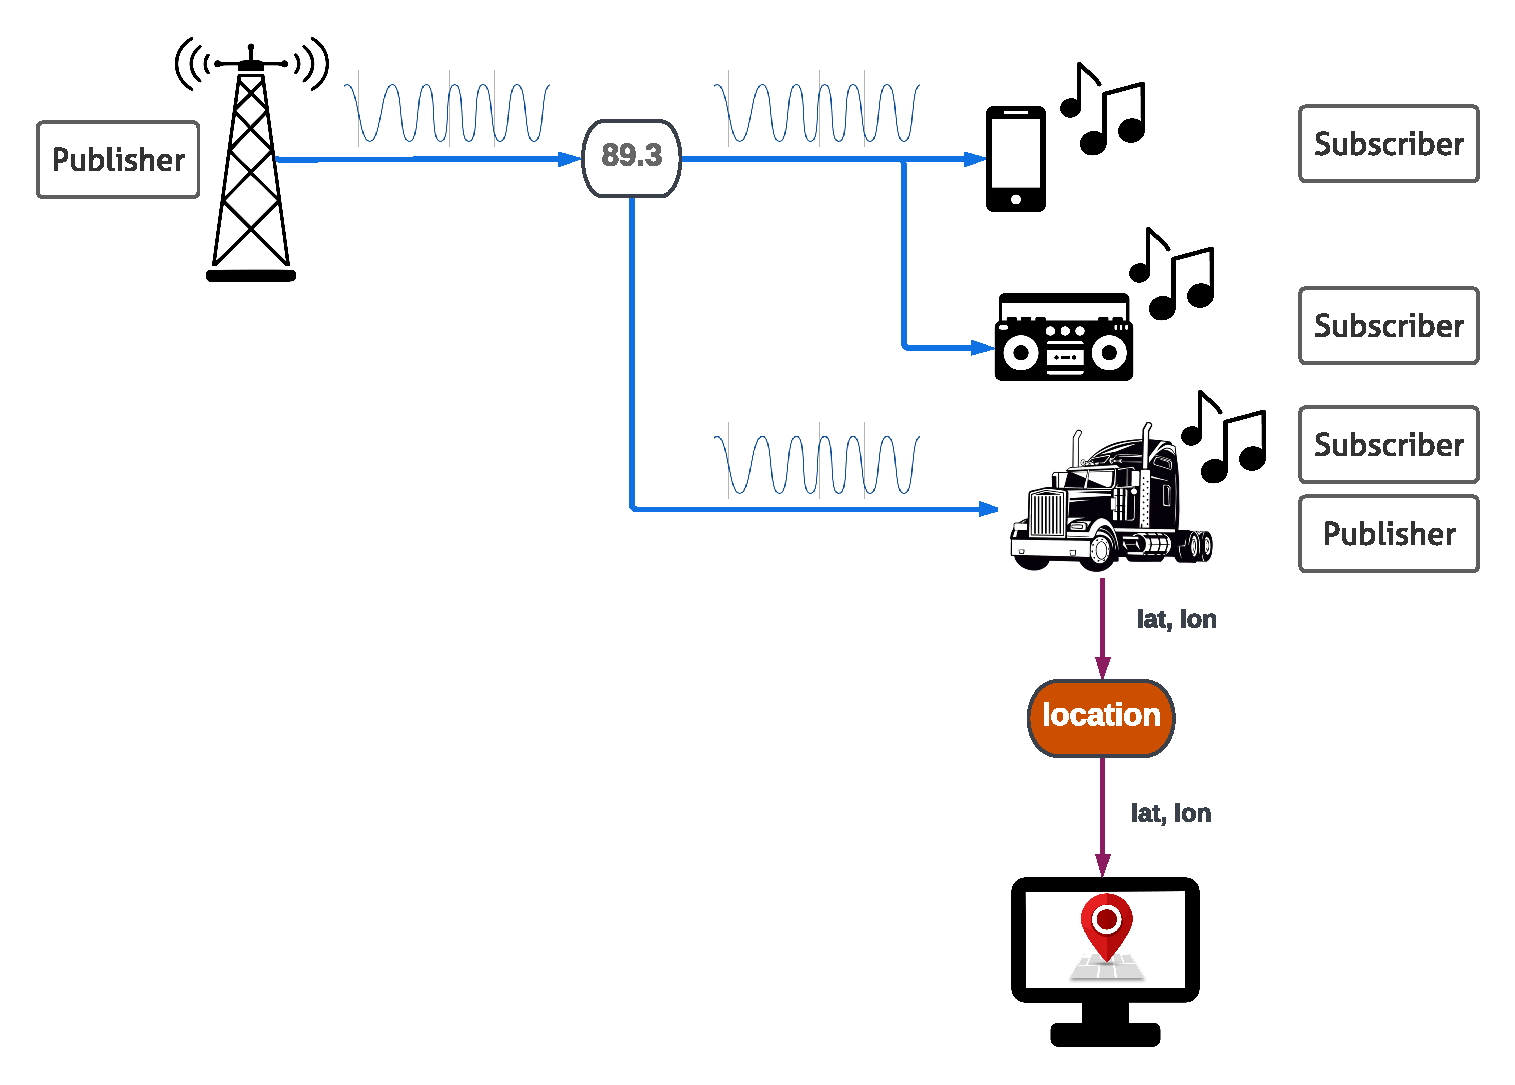
\includegraphics[width=.7\linewidth]{figures/lecture2/analogy9.pdf}

\end{center}
\vspace*{\fill}
\end{frame}


%=+=+=+=+=+=+=+=+=+=+=+=+=+=+=+=+=+=+=+=+=+=+=+=+=+=
\subsection{Summary}
\begin{frame}[fragile]{\secsec}
\vspace*{\fill}

{\large \mynote Summary} \doublerulefill

\begin{center} 

\begin{compactitem}
\item Publishers and subscribers must work with the same Message type.
\item The goal of Publishers is to only send Messages to Topics.
\item The goal of Subscribers is to only receive Messages from Topics.
\item There can be multiple Subscribers to a Topic. 
\item There can be multiple Publishers to the same Topic.
\item A Publisher can publish to different Topics.
\item A Node can be both a Publisher and a Subscriber.
\end{compactitem}

\end{center}
\vspace*{\fill}
\end{frame}

%%%%%%%%%%%%%%%%%%%%%%%%%%%%%%%%%%%%%%%%%%%%%%%%
\section{Running Nodes}
\begin{frame}[fragile]{\sec}
\vspace*{\fill}
\begin{center} 

{\large \mynote} \doublerulefill

There are mainly 2 ways to run Nodes in ROS.

\hrulefill

\begin{compactenum}
\item \myTool{ros2 run <package> <executable>} starts \emph{only} 1 Node.
\item \myTool{ros2 launch <package> <launch file>} starts \emph{at least} 1 Node, include other launch files, handles arguments, set parameters, etc.
\end{compactenum}
\end{center}
\vspace*{\fill}
\end{frame}


\subsection{ros2 run}
\begin{frame}[fragile]{\secsec}
\vspace*{\fill}
\begin{center} 
%%%%%%%%%%%%%%%%%%%%%%%%%%%%%%%%%%%%%%%%%%%%%%%%

{\large \mytodo Run only a single Node} \doublerulefill

\myTool{ros2 run <package> <executable>} --  <package> is the name of a ROS package and <executable> is the name of the executable from <package>.

\mynote An executable in \CC is the machine code of your program (after compiling and linking the source code). An executable in Python is a Python script (usually a \myFile{*.py} file) or a file generated from a Python script.

\hrulefill

\begin{compactitem}
\item ROS Galactic comes with the package \myROSPackage{demo_nodes_cpp} installed. 
\item This package includes a Publisher with the name \myNode{talker} and a Subscriber with the name \myNode{listener}
\item The Publisher can be started from the executable \textit{talker} and the Subscriber can be started from the executable \textit{listener}.
    \item In one terminal, run the Publisher with \myTerminal{ros2 run demo_nodes_cpp talker}
    \item In a different terminal, run the Subscriber with \myTerminal{ros2 run demo_nodes_cpp listener}
\end{compactitem}
\end{center}
\vspace*{\fill}
\end{frame}


\subsection{ros2 launch}
\begin{frame}[fragile]{\secsec}
\vspace*{\fill}
\begin{center} 
%%%%%%%%%%%%%%%%%%%%%%%%%%%%%%%%%%%%%%%%%%%%%%%%

{\large \mytodo Run a launch file} \doublerulefill

\myTool{ros2 launch <package> <launch file name>} --  <package> is the name of a ROS package and <launch file name> is the name of a launch file which belongs to <package>.

\hrulefill

\begin{compactitem}
\item A \urllink{https://docs.ros.org/en/foxy/Tutorials/Intermediate/Launch/Creating-Launch-Files.html}{launch file}  written in Python, XML, or YAML can start and stop different nodes as well as trigger and act on various events. 
\item The following command will start both the Publisher and the Subscriber.
\item[]\myTerminal{ros2 launch demo_nodes_cpp talker_listener.launch.py}
\end{compactitem}




\end{center}
\vspace*{\fill}
\end{frame}


\section{Introspecting Nodes and Topics}
\begin{frame}[fragile]{\sec}
\vspace*{\fill}
\begin{center} 
%%%%%%%%%%%%%%%%%%%%%%%%%%%%%%%%%%%%%%%%%%%%%%%%

{\large \myinfo Introspect Nodes and Topics} \doublerulefill


\hrulefill

\begin{compactenum}
\item \myTool{ros2 node <option> [node name]} provides different options to introspects Nodes. Some examples are:

\begin{compactitem}
\footnotesize
\item \myTool{ros2 node list} lists all running Nodes.
\item \myTool{ros2 node info <node name>} provides information for a given Node.
\end{compactitem}

\item \myTool{ros2 topic <option> [topic name]} provides different options to introspects Topics. Some examples are:
\begin{compactitem}
\footnotesize
\item \myTool{ros2 topic list} lists all running Topics. Add the option \myTool{-t} to get the type of each Topic.
\item \myTool{ros2 topic info <topic name>} provides information for a given Topic. Add the option \myTool{-v} for more information.
\item \myTool{ros2 topic find <message type>} list all Topics with the given Message type.
\item \myTool{ros2 topic echo <topic name>} displays Messages being published on <topic name>.
\item \myTool{ros2 topic hz <topic name>} displays the frequency at which Messages are published.
\end{compactitem}


\item \myTool{rqt_graph} visually shows the connections between Nodes and Topics.
\end{compactenum}
\end{center}
\vspace*{\fill}
\end{frame}

%%%%%%%%%%%%%%%%%%
%   --- FRAME
%%%%%%%%%%%%%%%%%%
\section{ROS Workspace}
\begin{frame}[fragile]{\sec}
\vspace*{\fill}
\begin{center} 
{\large \mydefinition Workspace} \doublerulefill

{\large \emph{A ROS workspace is a folder where you write all packages  needed to build a ROS2 application.}}

{\large \mytodo} \doublerulefill

\begin{compactitem}
\item Create a workspace anywhere you want and give it a name of your choice.
\item[]\myTerminal{mkdir -p \textasciitilde/enpm663_ws/src}
\begin{compactitem}
\item \mywarning The \myFolder{src} folder is where you will create your custom ROS packages or the ones you will clone from github.
\end{compactitem}
\item Build the workspace: \myTerminal{cd \textasciitilde/enpm663_ws} followed with \myTerminal{colcon build}
\begin{compactitem}
\item \mywarning You have to be in the root folder of the workspace to build it.
\item \mynote The build process looks at packages inside \myFolder{src}  and build them. As of now, there is no package in \myFolder{src} but some folders are generated.
\end{compactitem}
\end{compactitem}
\end{center}
\vspace*{\fill}
\end{frame}



\begin{frame}[fragile]{\sec}
\vspace*{\fill}
\begin{center} 


\begin{columns}[T]
    \begin{column}{0.3\textwidth}

\begin{forest}
  pic dir tree,
  pic root,
  for tree={% folder icons by default; override using file for file icons
    directory,
  },
  [\footnotesize enpm663_ws
    [\footnotesize~src]
    [\footnotesize~build]
    [\footnotesize~log ]
    [\footnotesize~install
    % [\footnotesize\myfile{local_setup.bash}, file]
    [\footnotesize setup.bash, file]
    [\footnotesize ..., file]
    ]

  ]
\end{forest}
    \end{column}
    
\begin{column}{0.7\textwidth}
\begin{compactitem}
\small
\item \myFolder{src} contains custom ROS packages. These packages can be the ones you created or external ones.
\item \myFolder{build} contains the intermediate build
products for each package. For instance, object files are created in this folder.
\item \myFolder{log} contains log files generated during the build process.
\item \myFolder{install} contains the final build products which can be used to run code, but relies on the presence of the source space. For instance, executable files and libraries are generated in this folder.
\begin{compactitem}
\item This folder contains the file \myFile{setup.bash} which you will need to source so that ROS can detect your custom packages in this workspace. 
\item \mytodo Add the command to source this file in your \myFile{bashrc} This command must come after sourcing your ROS distribution.

\end{compactitem}
\end{compactitem}
\end{column}
 \end{columns}
 
 
 
\end{center}
\vspace*{\fill}
\end{frame}


\begin{frame}[fragile]{\sec}
\vspace*{\fill}
\begin{center} 


\begin{compactitem}
\footnotesize
\item Edit \myFile{bashrc}
    \begin{bashScriptListLine}
source /opt/ros/galactic/setup.bash
source <path_to_worspace>/install/setup.bash 
source /usr/share/colcon_argcomplete/hook/colcon-argcomplete.bash
source /usr/share/colcon_cd/function/colcon_cd.sh
eval "$(register-python-argcomplete3 ros2)"
eval "$(register-python-argcomplete3 colcon)"
    \end{bashScriptListLine}

\item Edit \myFile{zshrc}
    \begin{bashScriptListLine}
source /opt/ros/galactic/setup.zsh
source <path_to_worspace>/install/setup.zsh 
source /usr/share/colcon_argcomplete/hook/colcon-argcomplete.zsh
source /usr/share/colcon_cd/function/colcon_cd.sh
eval "$(register-python-argcomplete3 ros2)"
eval "$(register-python-argcomplete3 colcon)"
    \end{bashScriptListLine}
    
\end{compactitem}

\end{center}
\vspace*{\fill}
\end{frame}


%%%%%%%%%%%%%%%%%%
%   --- FRAME
%%%%%%%%%%%%%%%%%%
\section{ROS Package}
\begin{frame}[fragile]{\sec}
\vspace*{\fill}
\begin{center} 
{\large \mydefinition Package} \doublerulefill

{\emph{Software in ROS is organized in packages. A package contains anything that logically constitutes a useful module. The goal of these packages it to provide this useful functionality in an easy-to-consume manner so that software can be easily reused.}}

\hrulefill

\begin{compactitem}
\footnotesize
\item Package creation in ROS2 uses \myTool{ament} as its build system and \myTool{colcon} as its build tool. 
\item  \myTool{ament} is an evolution of \myTool{catkin}
\item \myTool{ament} is a meta build system to improve building applications which are split into separate packages. It consists of two major parts:
\begin{compactitem}
\footnotesize
\item A build system to configure, build, and install a single package.
\item A tool to invoke the build of individual packages in their topological order. The tool relies on meta information about the packages to determine their dependencies and their build type. This meta information is defined in a manifest file called \myFile{package.xml} which is specified in \urllink{https://www.ros.org/reps/rep-0140.html}{REP 140}.
\end{compactitem}
\item More information on \myTool{ament} can be found \urllink{https://design.ros2.org/articles/ament.html}{here}.
\end{compactitem}
\end{center}
\vspace*{\fill}
\end{frame}


%%%%%%%%%%%%%%%%%%
%   --- FRAME
%%%%%%%%%%%%%%%%%%
\subsection{\CC}
\begin{frame}[fragile]{\secsec}
\vspace*{\fill}
\begin{center} 
{\normalsize \mytodo Create the \CC package \myROSPackage{first_package_cpp}} \doublerulefill

\begin{compactitem}
    \small
    \item \myreminder Packages are created in the \myFolder{src} folder of your workspace.
\end{compactitem}




\hrulefill
 
\begin{compactitem}
\footnotesize
\item \myTerminal{cd \textasciitilde/enpm663_ws/src}
\item \myTerminal{ros2 pkg create first_package_cpp -{}-build-type ament_cmake -{}-dependencies rclcpp}
\item or  \myTerminal{ros2 pkg create first_package_cpp  -{}-dependencies rclcpp}
\item \myTerminal{cd ..}
\item \myTerminal{colcon build}
\item \myTerminal{source install/setup.bash} 


\end{compactitem}

\hrulefill

\begin{compactitem}
\footnotesize

\item \mywarning Always source your workspace after building a new package for the first time.

\item \mynote To build a specific package: \myTerminal{colcon build -{}-packages-select <package name>}

\end{compactitem}
\end{center}
\vspace*{\fill}
\end{frame}


%*%*%*%*%*%*%*%*%*%*%*%*%*%*%*%*%*%*%*%*%*%*
\begin{frame}[fragile]{\secsec}
\vspace*{\fill}
\begin{center} 

\begin{columns}
\begin{column}{0.6\textwidth}

    \begin{itemize}
    \footnotesize
    \item \mydirFoot{first_package_cpp} -- This is the ROS package.
    \item \mydirFoot{include} -- \CC header files (.hpp) are expected to be placed in this folder.
    \item \mydirFoot{src} -- \CC source files (.cpp) are expected to be placed in this folder.
    \item \myfileFoot{CMakeLists.txt} contains rules to generate executables, libraries, and install folders and files.
    \item \myfileFoot{package.xml} contains meta information about the package.
        
        
        
        
        
    \end{itemize}

\end{column}
\begin{column}{0.4\textwidth}  %%<--- here
\begin{forest}
  pic dir tree,
  pic root,
  for tree={% folder icons by default; override using file for file icons
    directory,
  },
    [\small~first_package_cpp
     [\small~include]
      [\small~src]
    [\small CMakeLists.txt, file]
    [\small package.xml, file]
  ]
\end{forest}
\end{column}
\end{columns}
\end{center}
\vspace*{\fill}
\end{frame}


%*%*%*%*%*%*%*%*%*%*%*%*%*%*%*%*%*%*%*%*%*%*
\subsection{Python}
%*%*%*%*%*%*%*%*%*%*%*%*%*%*%*%*%*%*%*%*%*%*
\begin{frame}[fragile]{\secsec}
\vspace*{\fill}
\begin{center} 

{\normalsize \mytodo Create the Python package \mypackageNormal{first_package_py}} \doublerulefill

\myreminder Packages are created in \mydirNormal{\textasciitilde/enpm663_ws/src}


\hrulefill
 
\begin{compactitem}
\small
\item \myTerminal{cd \textasciitilde/enpm663_ws/src}
\item \myTerminal{ros2 pkg create first_package_py -{}-build-type ament_python -{}-dependencies rclpy}
\item \myTerminal{cd ..}
\item \myTerminal{colcon build}
\item \myTerminal{source install/setup.bash} 
\end{compactitem}
\end{center}
\vspace*{\fill}
\end{frame}

%*%*%*%*%*%*%*%*%*%*%*%*%*%*%*%*%*%*%*%*%*%*
\begin{frame}[fragile]{\secsec}
\vspace*{\fill}
\begin{center} 

\begin{columns}
\begin{column}{0.6\textwidth}

    \begin{itemize}
    \footnotesize
    \item \myFolder{first_package_py} -- This is your ROS package.
    \item \myFolder{first_package_py} -- Directory with the same name as your package. This is where you create your Nodes (Python scripts).
    \item \myFolder{resource} -- Folder which contains an empty file, with the same name as your package. In order to detect that a package is installed, ROS2 needs to install a marker file, which is the empty file inside \myFolder{resource}
    \item \myFolder{test} -- Folder which contains files to run test for your package.
        \item \myFile{package.xml} contains meta information about the package.
        \item \myFile{setup.py} contains instructions for how to install the package.
        \begin{itemize}
        \scriptsize
            \item \mynote Each time you add a Node in your package you need to edit this file.
        \end{itemize}
        \item \myFile{setup.cfg} is required when a package has executables, so \myTool{ros2 run} can find them.
        
        
        
    \end{itemize}

\end{column}
\begin{column}{0.4\textwidth}  %%<--- here
\begin{forest}
  pic dir tree,
  pic root,
  for tree={% folder icons by default; override using file for file icons
    l sep=5mm,
    l=0,
    directory,
  },
  [\scriptsize first_pkg_py 
    [\scriptsize~first_pkg_py
    [\scriptsize __init__.py, file]
    ]
    [\scriptsize~resource]
    [\scriptsize~test]
    [\scriptsize~package.xml, file]
    [\scriptsize~setup.py, file]
    [\scriptsize~setup.cfg, file]
    ]
\end{forest}
\end{column}
\end{columns}
\end{center}
\vspace*{\fill}
\end{frame}


%*%*%*%*%*%*%*%*%*%*%*%*%*%*%*%*%*%*%*%*%*%*
\subsection{Notes}
%*%*%*%*%*%*%*%*%*%*%*%*%*%*%*%*%*%*%*%*%*%*
\begin{frame}[fragile]{\secsec}
\vspace*{\fill}
\begin{center} 

{\large \mynote Python Packages} \doublerulefill

\begin{itemize}
    \item You can execute Python Nodes without building the Python package. However, when a package is built, colcon installs the Python scripts in a place where they can find other modules from other packages, where they can be found by other scripts. It will also allow you to start a node with \myTool{ros2 run}, add it in a launch file, pass parameters to it, etc.
    \item When \myTerminal{colcon build -{}-symlink-install} is used, building a Python package again is not required after editing a Python script.
\end{itemize}

\end{center}
\vspace*{\fill}
\end{frame}




%%%%%%%%%%%%%%%%%%
%   --- CPP and PYTHON 
%%%%%%%%%%%%%%%%%%
\subsection{\CC and Python}
\begin{frame}[fragile]{\secsec}
\vspace*{\fill}
\begin{center} 


{\normalsize \mytodo Create a package for both \CC and  Python:~ \myROSPackage{first_package}} \doublerulefill

\hrulefill

\begin{compactitem}
    \footnotesize
    \item To create a package which will contain both \CC and Python Nodes you first need to create a \CC package and then add folders and files to create a Python package.
\end{compactitem}
\begin{compactenum}
    \footnotesize
    \item Create a standard \CC package:
    \item[] \myTerminal{ros2 pkg create first_package -{}-build-type ament_cmake -{}-dependencies rclcpp rclpy}
    \item Create a Python package:
    \item[] \myTerminal{cd <path to first_package>}
    \item[] \myTerminal{mkdir first_package} -- This folder has the same name as the package. Python modules that need to be imported will be placed in this folder.
    \item[] \myTerminal{touch first_package/__init__.py} 
    \item[] \myTerminal{mkdir nodes} -- Python nodes will be placed in this folder.
\end{compactenum}

\hrulefill

{\normalsize \myreminder For this course you will need a package for \CC and Python Nodes}
\end{center}
\vspace*{\fill}
\end{frame}




\begin{frame}[fragile]{\secsec}
\vspace*{\fill}
\begin{center} 

\begin{forest}
  pic dir tree,
  pic root,
  for tree={% folder icons by default; override using file for file icons
    directory,
  },
    [\small~first_package
    [\small~first_package
    [\small __init__.py, file]
    ]
    [\small~nodes]
     [\small~include]
      [\small~src]
    [\small CMakeLists.txt, file]
    [\small package.xml, file]
  ]
\end{forest}
\end{center}
\vspace*{\fill}
\end{frame}

%%%%%%%%%%%%%%%%%%
%   --- FRAME
%%%%%%%%%%%%%%%%%%
\begin{frame}[fragile]{\sec}
\vspace*{\fill}
\begin{center} 

The tool \myTool{ros2 pkg list} provides a list of all visible package.

{\large \mytodo} \doublerulefill

Check the packages we created in this class are listed.
\begin{compactitem}
\item \myTerminal{ros2 pkg list | grep first_package}
\end{compactitem}

\end{center}
\vspace*{\fill}
\end{frame}

%%%%%%%%%%%%%%%%%%
%   --- FRAME
%%%%%%%%%%%%%%%%%%
\subsection{Package Manifest}
\begin{frame}[fragile]{\secsec}
\vspace*{\fill}
\begin{center} 
{\large \mynote} \doublerulefill

{\large The package manifest \myFile{package.xml} must be included with any
ROS-compliant package's root folder.}

\hrulefill
 
\begin{compactitem}
\item The package manifest has at least 3 purposes:
\begin{compactenum}
\item \myTool{ament} makes use of the manifest to build the dependency tree to determine build order. \item The manifest is used to install missing packages:
\begin{compactitem}
\item \myTerminal{cd \textasciitilde/ros2_ws}
\item \myTerminal{rosdep install -{}-from-paths ./src -{}-ignore-packages-from-source -y}

\end{compactitem}
\item Information on packages released to the ROS community is pulled from this file (see example with  \urllink{https://index.ros.org/p/rclcpp/#galactic-deps}{rclcpp}).
\end{compactenum}
\item \mynote If you are planning to release a ROS package to the community, edit \myFile{package.xml} with the correct information.
\end{compactitem}
\end{center}
\vspace*{\fill}
\end{frame}


%%%%%%%%%%%%%%%%%%
%   --- FRAME
%%%%%%%%%%%%%%%%%%
% \subsection{Build Script}
% \begin{frame}[fragile]{\secsec}
% \vspace*{\fill}
% \begin{center} 
% {\large \mynote} \doublerulefill

% {\large \myfileNormal{CMakeLists.txt} is used by \mytoolNormal{ament\_cmake} to build \CC executables, shared libraries (e.g., Gazebo plugins), and to install files in the folder \mydirNormal{install}}

% \hrulefill
 
% % \begin{compactitem}
% % \item \mytodo Take a look at the \urllink{https://docs.ros.org/en/foxy/How-To-Guides/Ament-CMake-Documentation.html}{documentation} for \mytoolSmall{ament_cmake}
% \begin{compactitem}
% \item \textcolor{black}{\texttt{cmake_minimum_required(VERSION 3.8)}} informs about the minimum version of \mytoolSmall{cmake} required to work with this file.
% \item The argument to \textcolor{black}{\texttt{project()}} will be the package name and must be identical to the package name in the \myfileSmall{package.xml}. 
% \item The project setup is done by \textcolor{black}{\texttt{ament_package()}} and this call must occur exactly once per package (more information \urllink{https://docs.ros.org/en/foxy/How-To-Guides/Ament-CMake-Documentation.html}{here}). 
% \item \mynote We need to edit this file once we create a Node in this package.
% \end{compactitem}

% \end{center}
% \vspace*{\fill}
% \end{frame}


%%%%%%%%%%%%%%%%%%
%   --- FRAME
%%%%%%%%%%%%%%%%%%
% \subsection{ROS Node}
% \begin{frame}[fragile]{\secsec}
% \vspace*{\fill}
% \begin{center} 
% {\large \mytodo} \doublerulefill

% {\large In the package \mypackageNormal{first_package} write a Node \mynodeNormal{hello} which prints ``Hello" in the terminal.}

% \hrulefill

% \begin{compactenum}
% \item Write a Node.
% \begin{compactitem}
% \item Create \myfileSmall{main.cpp} in \mydirSmall{first_package/src}
% \item Write the code for the Node in \myfileSmall{main.cpp}
% \item Edit \myfileSmall{CMakeLists.txt} to build and install the executable.
% \end{compactitem}
% \item Build the executable.
% \begin{compactitem}
% \item \myterminalSmall{cd \textasciitilde/ros2_ws}
% \item \myterminalSmall{colcon build -{}-packages-select first_package}
% \item \myterminalSmall{source \textasciitilde/ros2_ws/install/setup.bash} 
% \end{compactitem}

% \item Run the Node.
% \begin{compactitem}
% \item \mynote You can run a Node from anywhere on your system, there is no need to be in the workspace.
% % \item \mytoolSmall{ros2 run <package> <executable>}
% \item \myterminalSmall{ros2 run first_package hello}
% \end{compactitem}
% \end{compactenum}
% \end{center}
% \vspace*{\fill}
% \end{frame}






% %%%%%%%%%%%%%%%%%%
% %   --- FRAME
% %%%%%%%%%%%%%%%%%%

% \begin{frame}[fragile]{\secsec}
% \vspace*{\fill}
% \begin{center} 
% {\large \mynote rclcpp} \doublerulefill

% \begin{compactitem}
% \item \mfoot{rclcpp::init(argc, argv)} initializes any global resources needed by the middleware and the client library, as well as doing client library related command line argument parsing. 
% \item \mfoot{rclcpp::shutdown()} causes all Nodes and their constituent parts to become invalid and shutdown. It also destroys any global resources created when \mfoot{rclcpp::init(argc, argv)}  was originally called.
% \begin{compactitem}
% \item By default \mfoot{rclcpp} also installs a SIGINT handler which will detect \mykbFoot{ctrl-c} and automatically shut down for you. 
% \end{compactitem}
% \item See \urllink{https://docs.ros2.org/alpha8/rclcpp_cpp_client_library_overview.html#shutdown-and-reinitialization}{Documentation} for \mytoolSmall{rclcpp}
% \end{compactitem}

% \end{center}
% \vspace*{\fill}
% \end{frame}


% %%%%%%%%%%%%%%%%%%
% %   --- FRAME
% %%%%%%%%%%%%%%%%%%

% \subsubsection*{ROS Logging}
% \begin{frame}[fragile]{\secsecsec}
% \vspace*{\fill}
% \begin{center} 
% {\large \mynote ROS Logging} \doublerulefill

% \begin{compactitem}
% \item Although \mfoot{std::cout} works in ROS, it is not the appropriate way to print messages in the terminal.
% \item ROS uses a \urllink{https://docs.ros.org/en/foxy/Concepts/About-Logging.html}{logging} mechanism with different severity levels. 
% \item Each Node has a logger associated with it that automatically includes the Node's name and namespace. 
% \item The logging subsystem in ROS2 aims to deliver logging messages to a variety of targets, including:
% \begin{compactitem}
% \item To the terminal.
% \item To log files on disk, located in \mydirSmall{\textasciitilde/.ros/log}
% \item To the Topic \mytopicSmall{/rosout}
% \end{compactitem}

% \end{compactitem}

% \end{center}
% \vspace*{\fill}
% \end{frame}

% \begin{frame}[fragile]{\secsecsec}
% \vspace*{\fill}
% \begin{center} 
% {\large \mynote ROS Logging} \doublerulefill

% \begin{compactitem}
% \item The different severity levels in ROS are:
% \begin{compactitem}
% \item \mfoot{DEBUG}: This severity level should only be used during debugging. It should not be used in the released version of the package (it should not be used in submitted assignments).
% \item \mfoot{INFO}: Small amounts of information that may be useful to a user.
% \item \mfoot{WARN}: Information that the user may find alarming, and may affect the output of
% the application, but is part of the expected working of the system (e.g., ``robot too close to human").
% \item \mfoot{ERROR}: Something serious (but recoverable) has gone wrong (e.g., ``robot controllers shut down temporarily").
% \item \mfoot{FATAL}: Something unrecoverable has happened (e.g., ``the world just imploded").
% \end{compactitem}
% \item Each severity level can be used with 14 different functions.
% \end{compactitem}

% \end{center}
% \vspace*{\fill}
% \end{frame}

% %%%%%%%%%%%%%%%%%%
% %   --- FRAME
% %%%%%%%%%%%%%%%%%%
% \subsubsection*{Edit CMakeLists.txt}
% \begin{frame}[fragile]{\secsecsec}
% \vspace*{\fill}
% \begin{center} 
% {\large \mytodo Edit CMakeLists.txt} \doublerulefill

% \begin{compactitem}
% \item You need to edit \myfileSmall{CMakeLists.txt} to build and install the executable.

% \begin{cmakescript}
% add_executable(hello src/main.cpp)
% ament_target_dependencies(hello rclcpp)

% install(TARGETS
%   hello
%   DESTINATION lib/${PROJECT_NAME}
% )
% \end{cmakescript}

% \end{compactitem}

% \end{center}
% \vspace*{\fill}
% \end{frame}


% \subsubsection*{Spinning a Node}
% \begin{frame}[fragile]{\secsecsec}
% \vspace*{\fill}
% \begin{center} 
% {\large \mydefinition Spinning a Node} \doublerulefill


% \begin{compactitem}
% \item \mfoot{rclcpp::spin(node)} pauses the program to keep your Node alive. 
% \item Without this function, the Node will execute the instructions and shuts down by itself.
% \item Usually we would like to keep a Node running while the robot is still working.
% \item \mynote \mfoot{rclcpp::spin(node)} only takes a shared pointer as argument and this is why we used a shared pointer in the program we wrote.
% \end{compactitem}

% \end{center}
% \vspace*{\fill}
% \end{frame}


% \subsubsection*{OOP}
% \begin{frame}[fragile]{\secsecsec}
% \vspace*{\fill}
% \begin{center} 


% \begin{compactitem}
% \item The code we wrote is fine for a simple Node.
% \item Nodes usually need to publish Messages and/or receive Messages.
% \item Messages need to be stored as Message objects to be processed later.
% \item OOP is a good solution for such complexity.
% \begin{compactitem}
% \item See a curated list of  \urllink{https://github.com/fkromer/awesome-ros2}{ROS2 projects} with examples using OOP.
% \end{compactitem}
% \end{compactitem}

% {\large \mytodo} \doublerulefill

% \begin{compactitem}
% \item Rewrite the Node using OOP.
% \item If \myfileSmall{*.h} files are created, you need to edit  \myfileSmall{CMakeLists.txt} so they can be found and installed.
% \begin{cmakescript}
% include_directories(
%   include/first_package
% )

% install(DIRECTORY
%         include
%         DESTINATION share/${PROJECT_NAME})
% \end{cmakescript}
% \end{compactitem}

% \end{center}
% \vspace*{\fill}
% \end{frame}



% \begin{frame}[fragile]{\secsecsec}
% \vspace*{\fill}
% \begin{center} 
% {\large \mytodo} \doublerulefill



% \begin{compactitem}
% \item Zip \mypackageSmall{first_package} and then delete the package.
% \item Delete the folders \mydirSmall{log}, \mydirSmall{build}, and \mydirSmall{install}
% \item Clone the folder \mydirSmall{enpm809y_fall2022} in \mydirSmall{\textasciitilde/ros2_ws/src}
% \item \myterminalSmall{cd \textasciitilde/ros2_ws/src}
% \item \myterminalSmall{git clone https://github.com/zeidk/enpm809y_fall2022.git}
% \end{compactitem}

% \end{center}
% \vspace*{\fill}
% \end{frame}

%%%%%%%%%%%%%%%%%%
%   --- FRAME
%%%%%%%%%%%%%%%%%%
\section{Function for Sourcing a Specific Package}
\begin{frame}[fragile]{\sec}
\vspace*{\fill}
\begin{center} 

\begin{bashScriptList}
# define the function
function enpm663(){
  source /opt/ros/galactic/setup.zsh
  cd /home/zeid/dev/enpm663_ws
  source install/setup.zsh
  export _colcon_cd_root=/home/zeid/dev/enpm663_ws
  source /usr/share/colcon_argcomplete/hook/colcon-argcomplete.zsh
  source /usr/share/colcon_cd/function/colcon_cd.sh
  eval "$(register-python-argcomplete3 ros2)"
  eval "$(register-python-argcomplete3 colcon)"
}

# call the function
enpm663
\end{bashScriptList}

\end{center}
\vspace*{\fill}
\end{frame}




%%%%%%%%%%%%%%%%%%
%   --- FRAME
%%%%%%%%%%%%%%%%%%
\section{Next Class}
\begin{frame}[fragile]{\sec}
\vspace*{\fill}
\begin{center} 

{\large \myinfo \cnordZero{L2:} Course Introduction} \doublerulefill

{\large \mywarning Quiz} \doublerulefill

\end{center}
\vspace*{\fill}
\end{frame}
%=+=+=+=+=+=+=+=+=+=+=+=+=+=+=+=+=+=+=+=+=+=+=+=+=+=+=+=+=+=+=+=+=+=+=+=+=+=+=+=
% END OF DOCUMENT
%=+=+=+=+=+=+=+=+=+=+=+=+=+=+=+=+=+=+=+=+=+=+=+=+=+=+=+=+=+=+=+=+=+=+=+=+=+=+=+=
\end{document}